\documentclass[a4paper,12pt]{article}
\usepackage[a4paper,margin=1in]{geometry}
\usepackage{graphicx}
\usepackage{amsmath, amssymb}
\usepackage{hyperref}
\usepackage{cite}
\usepackage{authblk}
\usepackage{float}
\usepackage{microtype}
\usepackage{verbatim}
\usepackage{natbib}
\usepackage{subcaption}
\graphicspath{ {./images/} }

\title{Spatial Deconvolution of Pro-Angiogenic Endothelial Cells in Human Atherosclerotic Plaques Using Cell2Location}

\author[1,2]{T. Truc Bui}
\author[1,2]{Max-Malte Hansen}
\author[1,2]{Jan P. Hummel}
\author[1,2]{Julius J. Stein}
\author[3]{Korbinian Träuble}

\renewcommand{\Affilfont}{\small} % Change affiliation size

\affil[1]{Department of Computer Science, TUM School of Computation, Information and Technology, Technical University of Munich, Garching, Germany}
\affil[2]{Faculty of Mathematics, Computer Science and Statistics, Ludwig Maximilian University of Munich, Munich, Germany}
\affil[3]{Institute of Computational Biology, German Research Center for Environmental Health, Helmholtz Zentrum München, Neuherberg, Germany}

\date{\today}

%TODO: add outline

\begin{document}
\maketitle

%TODO: add results to abstract section
\begin{abstract}
Atherosclerosis is a progressive disease involving complex cellular and molecular interactions within arterial plaques, ultimately leading to plaque growth and potential plaque rupture. Recent single-cell and spatial transcriptomic studies highlight the heterogeneity of cells contributing to disease progression, yet the precise localization of specialized endothelial cell (EC) subtypes remains elusive. Here, we leverage Cell2Location \cite{Kleshchevnikov2022-vd}, a robust Bayesian deconvolution method, to integrate a comprehensive single-cell RNA sequencing (scRNA-seq) reference from an atherosclerosis plaque atlas \cite{Traeuble2024-de} with Visium spatial transcriptomic data \cite{Bleckwehl2025-td} obtained from 12 human coronary artery samples. Our analyses focus on the distribution of pro-angiogenic endothelial cells (ECs), a subset known to promote neovascularization and potentially influence plaque progression. By applying Cell2Location to 16,593 spatial spots, we systematically quantify cell-type abundances and reveal distinct spatial patterns of pro-angiogenic ECs across varying plaque stages. We further show that these cells localize in close proximity to macrophage- and smooth muscle cell–rich regions, underscoring potential crosstalk involved in neovessel formation and lesion remodeling. These findings offer novel insights into the tissue microarchitecture of atherosclerotic plaques and highlight the importance of pro-angiogenic ECs as potential therapeutic targets for disease intervention.
\end{abstract}

% TODO: add references
\section{Introduction}
Atherosclerosis is characterized by the accumulation of lipids and immune cells in arterial walls, leading to plaque formation. Recent advancements in spatial transcriptomics allow for high-resolution mapping of cell types within these lesions. This study aims to determine the spatial distribution of pro-angiogenic ECs using Visium spatial transcriptomics and Cell2Location.

Atherosclerosis is a chronic inflammatory disease characterized by the buildup of lipids, immune cells, and fibrous elements in arterial walls, resulting in plaque formation that can narrow or obstruct blood flow. Over time, progressive accumulation of these components can lead to plaque instability, which poses a risk for acute thrombotic events such as myocardial infarction or stroke. Traditional profiling approaches, such as bulk RNA sequencing or immunohistochemistry, have provided crucial insights into the cellular composition of atherosclerotic lesions but lack the spatial resolution to disentangle the complex microenvironment within the plaque.

Recent advancements in spatial transcriptomics have enabled high-resolution mapping of gene expression in intact tissue sections, revealing how different cell types organize and interact within pathological niches. By combining single-cell RNA sequencing (scRNA-seq) data with spatially resolved expression profiles, researchers can pinpoint the location of transcriptionally defined cell subtypes and study their roles in disease progression. This is especially relevant in atherosclerosis, where numerous vascular and immune cell populations dynamically shape lesion development.

Pro-angiogenic endothelial cells (ECs) have emerged as key drivers of neovascularization in atherosclerotic plaques. These cells can sprout new vessels that infiltrate lesions, supplying additional oxygen and nutrients but potentially destabilizing plaques through increased permeability and inflammatory cell infiltration. Despite their recognized importance, the precise spatial distribution and the local microenvironmental cues influencing these cells have remained incompletely understood. Addressing this knowledge gap is critical, as therapeutic strategies that modulate plaque-associated angiogenesis could hold promise for stabilizing or even regressing atherosclerotic lesions.

Visium spatial transcriptomics, developed by 10x Genomics, provides high-throughput gene expression measurements at defined spots within the tissue. By overlaying histological information with spot-level RNA counts, one can identify distinct plaque regions—such as the fibrous cap, lipid core, and adventitia—and study the cellular composition in each. However, these spot-level data typically contain mixtures of multiple cell types, prompting the need for computational deconvolution methods to parse out the contributions of various cell populations. Cell2Location \citep{Kleshchevnikov2022-vd} addresses this challenge by leveraging gene expression signatures inferred from scRNA-seq to estimate absolute cell-type abundances in each spatial spot, thus enabling higher-resolution insights into tissue organization.

In this study, we integrate Visium spatial transcriptomic data from human coronary artery samples at different stages of atherosclerosis with a large, harmonized scRNA-seq reference atlas of plaque-associated cell types \citep{Traeuble2024-de}. We employ Cell2Location to (1) accurately estimate the spatial abundance of diverse immune and vascular cell types, including specialized EC subsets, and (2) systematically map the distribution of pro-angiogenic ECs within and across plaque regions. We hypothesize that pro-angiogenic ECs exhibit distinct spatial patterns, being enriched in neovascularized or inflamed plaque areas, thereby contributing to both vascular remodeling and lesion progression. By elucidating these spatial dynamics, we provide a refined view of endothelial heterogeneity that may guide future mechanistic and therapeutic studies in atherosclerosis.
\begin{comment}

\begin{itemize}
  \item Background on atherosclerosis and the significance of spatial transcriptomics.
  \item Role of pro-angiogenic endothelial cells (ECs) in plaque progression.
  \item Overview of Visium spatial transcriptomics and single-cell RNA sequencing (scRNA-seq).
  \item Introduction to Cell2Location as a computational tool for spatial deconvolution.
  \item Hypothesis: Where are the pro-angiogenic ECs located spatially within atherosclerotic plaques?
\end{itemize}

\end{comment}

\section{Methods}
\subsection{Data Sources}
We utilize spatial transcriptomic data from Sikander Hayat’s Visium dataset and a reference scRNA-seq atlas of atherosclerotic plaques.

Hayat’s study applied Visium spatial transcriptomics to examine 12 human coronary arteries at different stages of atherosclerosis, capturing 16,593 spots with an average of 1,563 genes per spot. The dataset includes samples classified as Fibroatheroma (FW104302, FW104306), Atheroma (FW104860, FW106005\_v2, FW106014, FW106016, FW106022), Intermediate lesion (FW106006, FW106008), and Control (FW106010, FW106012, FW106018).

The single-cell RNA sequencing reference dataset from the Atherosclerosis Plaque scRNA-seq Atlas provides a comprehensive view of human atherosclerotic plaques by integrating %259,493 high-quality
259721
 annotated cells from carotid, coronary, and femoral arteries across all publicly available single-cell datasets. The dataset ensures robust cell type annotations validated by expert consensus and surface protein measurements. Cell types are categorized into level 1 annotations, which include broad groups such as Endothelial cells (ECs), Macrophages, T cells, and Dendritic cells, while level 2 annotations provide further granularity across these groups. This dataset enables accurate automatic cell type annotation of new scRNA-seq datasets and facilitates bulk RNA-seq deconvolution.

\subsection{Preprocessing and Quality Control}
Cell2Location is a computational framework designed to integrate single-cell RNA sequencing (scRNA-seq) data with spatial transcriptomics to infer the spatial distribution of fine-grained cell types in tissue sections. The tool takes reference cell type signatures derived from scRNA-seq and spatial transcriptomics data as input. In particular, the model takes an untransformed spatial expression count matrix of genes g={1,...,G} at locations s={1,...,S} as the first input. The second input is a matrix of reference cell type signatures, which correspond to the expected mRNA count of genes g for each cell type. Since the tool requires raw counts, we did not normalize the data but instead used the raw counts directly. 

The workflow begins with preprocessing of the scRNA-seq reference data. First, we filtered out cells with zero counts. Then, we applied gene filtering based on the following criteria: a minimum cell count cutoff of 1, a cell percentage cutoff of 0.03, and an average expression cutoff of 1.12 for non-zero cells. The pre-processed reference data consists of 259720 cells and 12615 genes.

The provided Visium dataset had already been deconvoluted; therefore, we first removed the existing results before mapping the data to the new atlas reference.

\subsection{Estimation of reference cell type signatures}

The second step is the estimation of reference cell type signatures, where Cell2Location applies negative binomial (NB) regression to infer the expected expression of each gene per cell type while accounting for variations in sequencing depth and batch effects.

Since we are interested in Pro-Angiogenic Endothelial
Cells, we focused on the level 2 cell type annotation. We built two different regression models for the reference data, both using the donor ID as the batch key and level 2 cell type annotations as the labels key. One model additionally included Assay as a categorical covariate. The models were trained for 250 epochs using GPU acceleration. After training, we summarized the posterior distribution and exported the estimated cell abundances to the reference data.

\subsection{Spot Deconvolution and Cell type mapping}

Once the reference signatures were established, we proceeded with cell type mapping, where the inferred cell-type signatures were projected onto the spatial transcriptomics dataset. This process involved deconvolution of the spatially resolved bulk RNA counts into estimated proportions of each cell type across spatial locations using Cell2Location’s Bayesian model.

We first identified shared genes (intersection) between the reference dataset and the Visium dataset to ensure compatibility. The model was then set up with the 12 different Visium samples as the batch key, using the following hyperparameters:

\begin{itemize}
    \item{Number of cells per location: 5, 7, and 10 (evaluated separately), chosen based on the expected number of cells per spot in Visium data.}
    \item{Regularization strength (detection\_alpha): 200}
\end{itemize}

Each configuration was trained for 30,000 epochs using GPU acceleration. We assessed the impact of varying the number of cells per location by comparing the resulting spatial distributions of key cell types, particularly Pro-Angiogenic Endothelial Cells.

To evaluate model performance, we examined the consistency of spatial patterns with known histopathological features of atherosclerosis. Among the tested values, 10 yielded the most biologically meaningful results, aligning with prior histological findings. Therefore, we selected this configuration for further downstream analysis and visualization.

\begin{comment}
 
Cell2Location, a Bayesian model, was applied to map scRNA-seq-derived cell types onto spatial spots, estimating cell type proportions within plaque regions.

The algorithm borrows statistical strength across spatial locations, enhancing the sensitivity to detect rare and fine-grained cell populations. This step is crucial for accurately identifying the tissue microarchitecture and understanding the spatial organization of cell types in complex tissues such as atherosclerotic plaques. Following mapping, the post-processing step involves visualization and interpretation of the spatial distribution of inferred cell types. Researchers can explore spatial co-localization patterns, validate findings against histological data, and perform downstream analyses such as ligand-receptor interaction studies to infer cell-cell communication. One of the key advantages of Cell2Location is its ability to analyze datasets from multiple experiments jointly, correcting for technical variability and increasing the robustness of cell type deconvolution. Additionally, the framework allows for estimation of absolute cell-type abundances rather than just relative proportions, providing deeper biological insights into tissue composition. The methodology has been applied successfully in a range of tissues, including brain, lymph nodes, and gut, where it has enabled the discovery of rare and spatially restricted cell populations. In the context of atherosclerosis research, Cell2Location can be leveraged to determine the spatial positioning of pro-angiogenic endothelial cells (ECs) within plaques, helping to understand their role in vascular remodeling and disease progression. The workflow provides a powerful tool for linking single-cell transcriptomics with spatial transcriptomics data, ultimately facilitating a more comprehensive understanding of tissue biology in both health and disease.

\begin{itemize}
  \item Explanation of Bayesian modeling in Cell2Location.
  \item Mapping scRNA-seq cell types onto spatial spots.
  \item Statistical validation of deconvolution results.
\end{itemize}

\end{comment}


\subsection{Spatial Localization and Functional Analysis}

Following mapping, the post-processing step involves visualization and interpretation of the spatial distribution of inferred cell types. We used the function \textit{pl.spatial()} from the package SCANPY \citep{scanpy} to visualize the proportion of Pro-Angiogenic ECs and EndoMT ECs across each slide. Additionally, we examined T cells (CD4+ and CD8+) and Macrophages (including HMOX1+ Macrophages, Inflammatory Macrophages, and other subtypes) to identify key immune cell distributions within the tissue.

TODO: What did we do here further?

\begin{comment}
We analyzed the localization of pro-angiogenic ECs, their co-localization with other vascular and immune cells, and performed pathway enrichment analyses to identify angiogenesis-related genes.

\begin{itemize}
  \item Identification of pro-angiogenic ECs in plaque regions.
  \item Co-localization with other vascular and immune cell types.
  \item Comparison across different plaque stages.
  \item Gene expression signatures of pro-angiogenic ECs.
  \item Enrichment analysis of angiogenic and inflammatory pathways.
  \item Cell-cell interaction analysis using ligand-receptor pairing (e.g., VEGF signaling).
\end{itemize}

\end{comment}

\newpage

\section{Results}

%TODO: add plots
%TODO: use N_cells 10 plots
\subsection{Spatial Deconvolution Reveals Distinct Cellular Landscapes in Healthy vs.\ Atherosclerotic Arteries}
We performed Cell2Location deconvolution on Visium spatial transcriptomic data derived from healthy (control) and atherosclerotic arterial samples. These samples included intermediate lesions, atheromas, and fibroatheromas, each displaying characteristic morphological features of progressive disease. By mapping eight key cell populations—EndoMT ECs, pro-angiogenic ECs, CD4 T cells, CD8 T cells, HMOX1\textsuperscript{+} macrophages, inflammatory macrophages, PLIN2\textsuperscript{+}/TREM1\textsuperscript{+} macrophages, and other macrophages—we captured a detailed landscape of tissue composition at the spot level. In controls, the vessel wall was generally thin and uniform, while atherosclerotic lesions showed substantial intimal thickening, plaque formation, and local necrosis or fibrosis. The color-coded probability maps produced by Cell2Location showed site-specific enrichments of immune or endothelial cell subtypes, reflecting the distinct microenvironments that develop as atherosclerosis advances. (Appendix C)

\subsection{Control Samples Exhibit Low Immune Infiltration and Quiescent Endothelium}
In control arteries, the thin tunica intima and well-defined lumen were accompanied by minimal cellular accumulations beyond the typical adventitial layer. EndoMT EC and pro-angiogenic EC signals were modest and largely confined to the luminal border, consistent with quiescent endothelium. CD4 and CD8 T-cell signatures were similarly low, appearing sporadically in adventitial regions, which is expected for normal immune surveillance (Figure 1). Macrophages displayed a low-intensity pattern as well, with sporadic detection of oxidative-stress–associated (HMOX1\textsuperscript{+}) or inflammatory phenotypes. This overall profile suggested that control vessels maintained a stable, low-inflammatory state that provided a baseline for subsequent comparisons with diseased samples.


\begin{figure}[H]
\centering
\begin{subfigure}{0.4\textwidth}
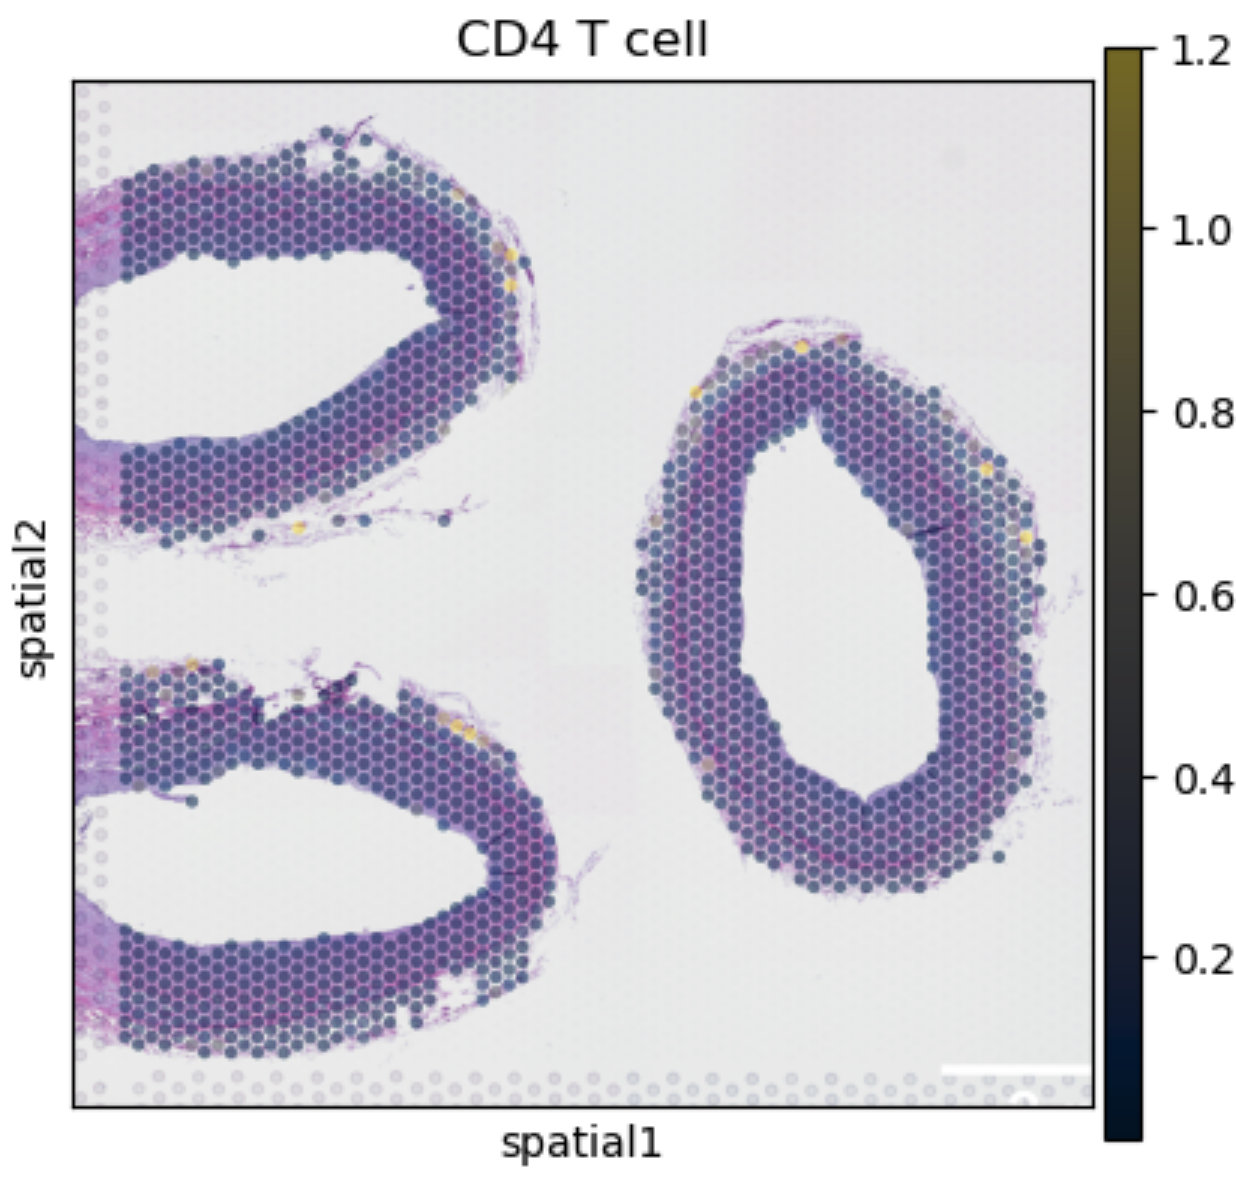
\includegraphics[width=\textwidth]{cd4pa2}
\caption{CD4 T-cell signature}
\label{fig:control_spatial}
\end{subfigure}
\hfill
\begin{subfigure}{0.4\textwidth}
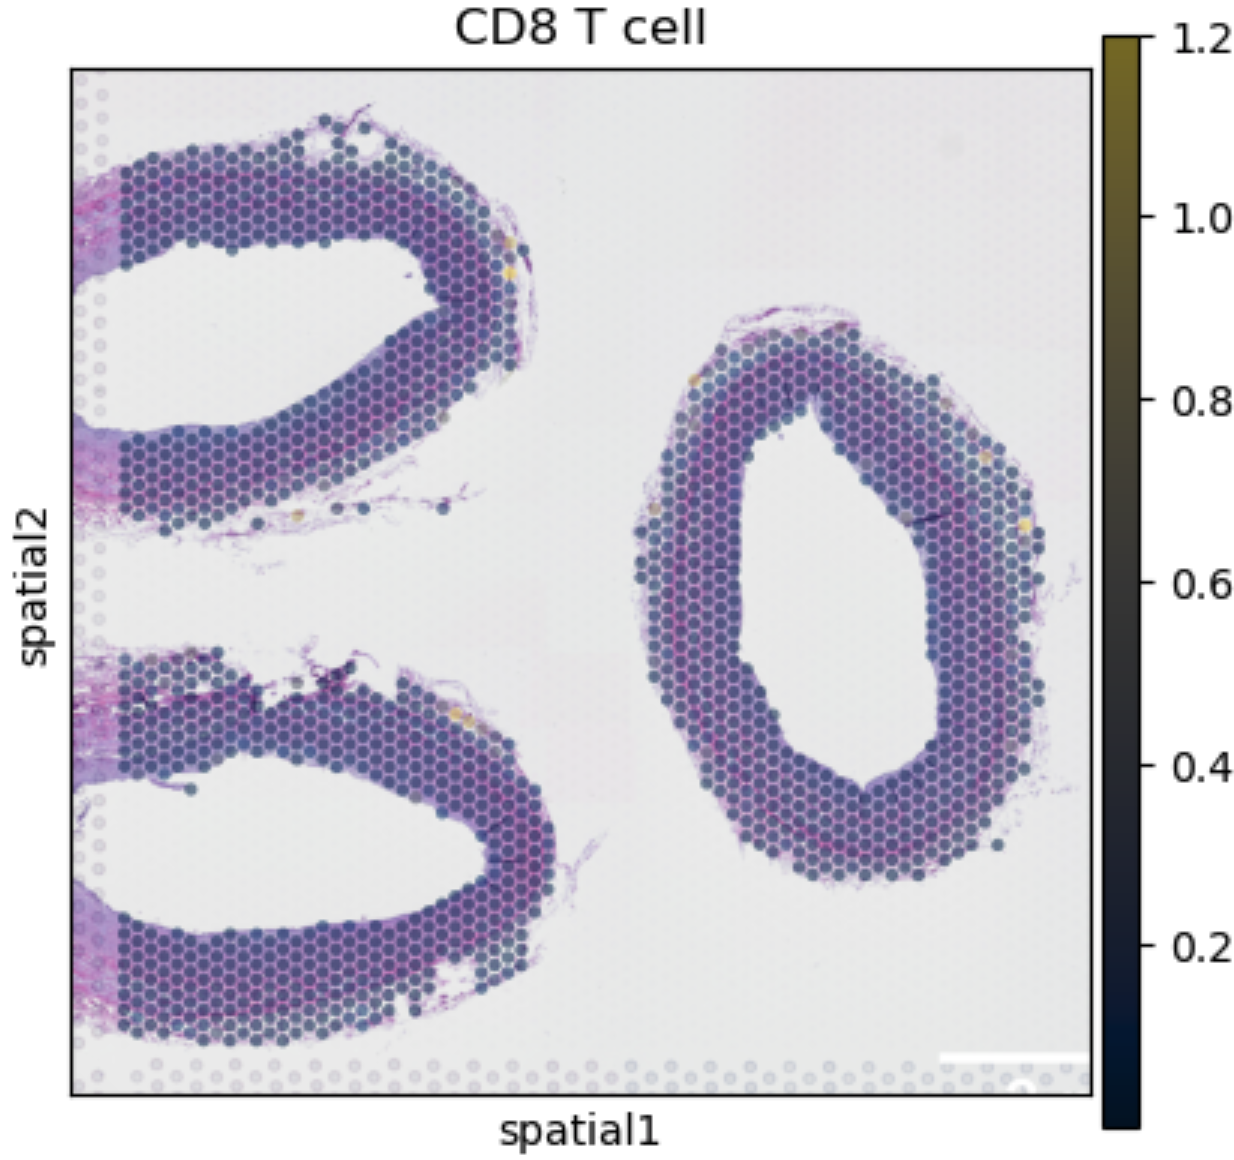
\includegraphics[width=\textwidth]{cd8pa3}
\caption{CD8 T-cell signature}
\label{fig:atherosclerosis_spatial}
\end{subfigure}
\caption{Low-Inflammatory state in control samples}
\label{fig:spatial_deconvolution}
\end{figure}

\subsection{Intermediate Lesions Show Emerging Neovascularization and Immune Infiltration}
In tissues classified as intermediate lesions, focal thickening of the intima and modest immune recruitment were readily apparent. Pro-angiogenic EC signals appeared elevated relative to controls, often at the interface of the intima and the media, suggesting early neovascular sprouts into regions experiencing hypoxia or inflammation (Figure 2). Small clusters of inflammatory and HMOX1\textsuperscript{+} macrophages localized beneath these nascent plaques, indicating an oxidative-stress response and the onset of lesion-associated inflammation. CD4 and CD8 T cells also increased slightly but did not form large, dense accumulations. These observations underscore the transitional stage in which quiescent arteries begin to exhibit localized endothelial remodeling and immune involvement, setting the stage for more advanced disease phenotypes.

MACHT DAS SINN BZW SIOND DIE PLTS HIER DURHCEINENDERGEKOMMEN/FALSCHB @JULIUS
\begin{figure}[H]
\centering
\begin{subfigure}{0.4\textwidth}
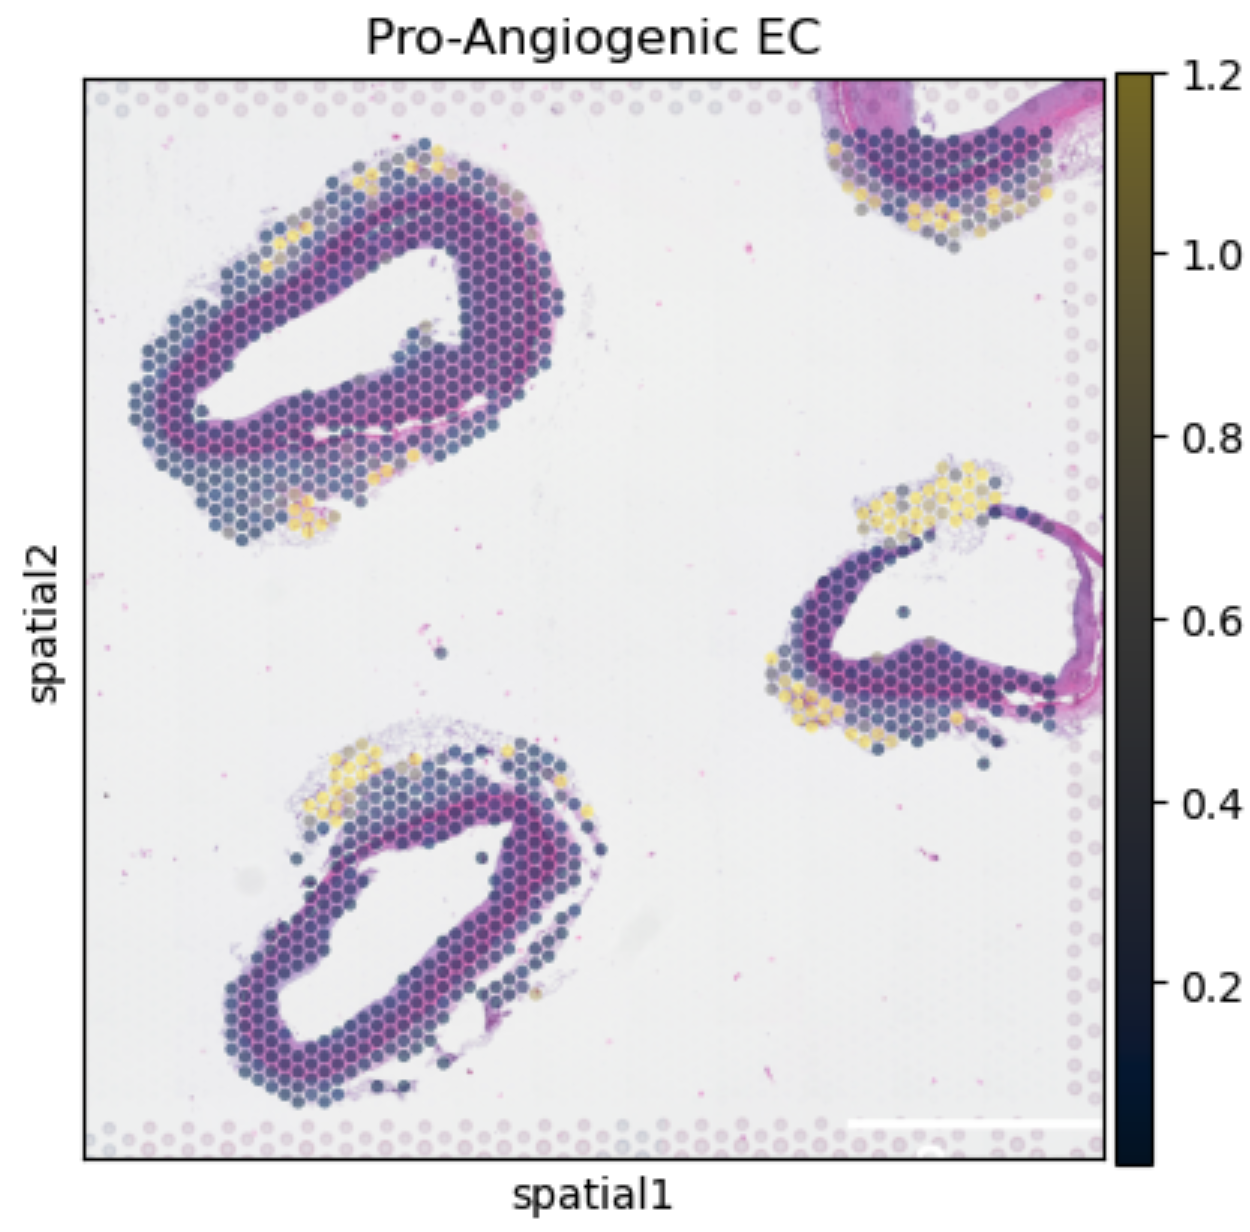
\includegraphics[width=\textwidth]{paecpa10}
\caption{Pro-Angiogenic EC signature in FW106010 control sample}
\label{fig:control_spatial}
\end{subfigure}
\hfill
\begin{subfigure}{0.4\textwidth}
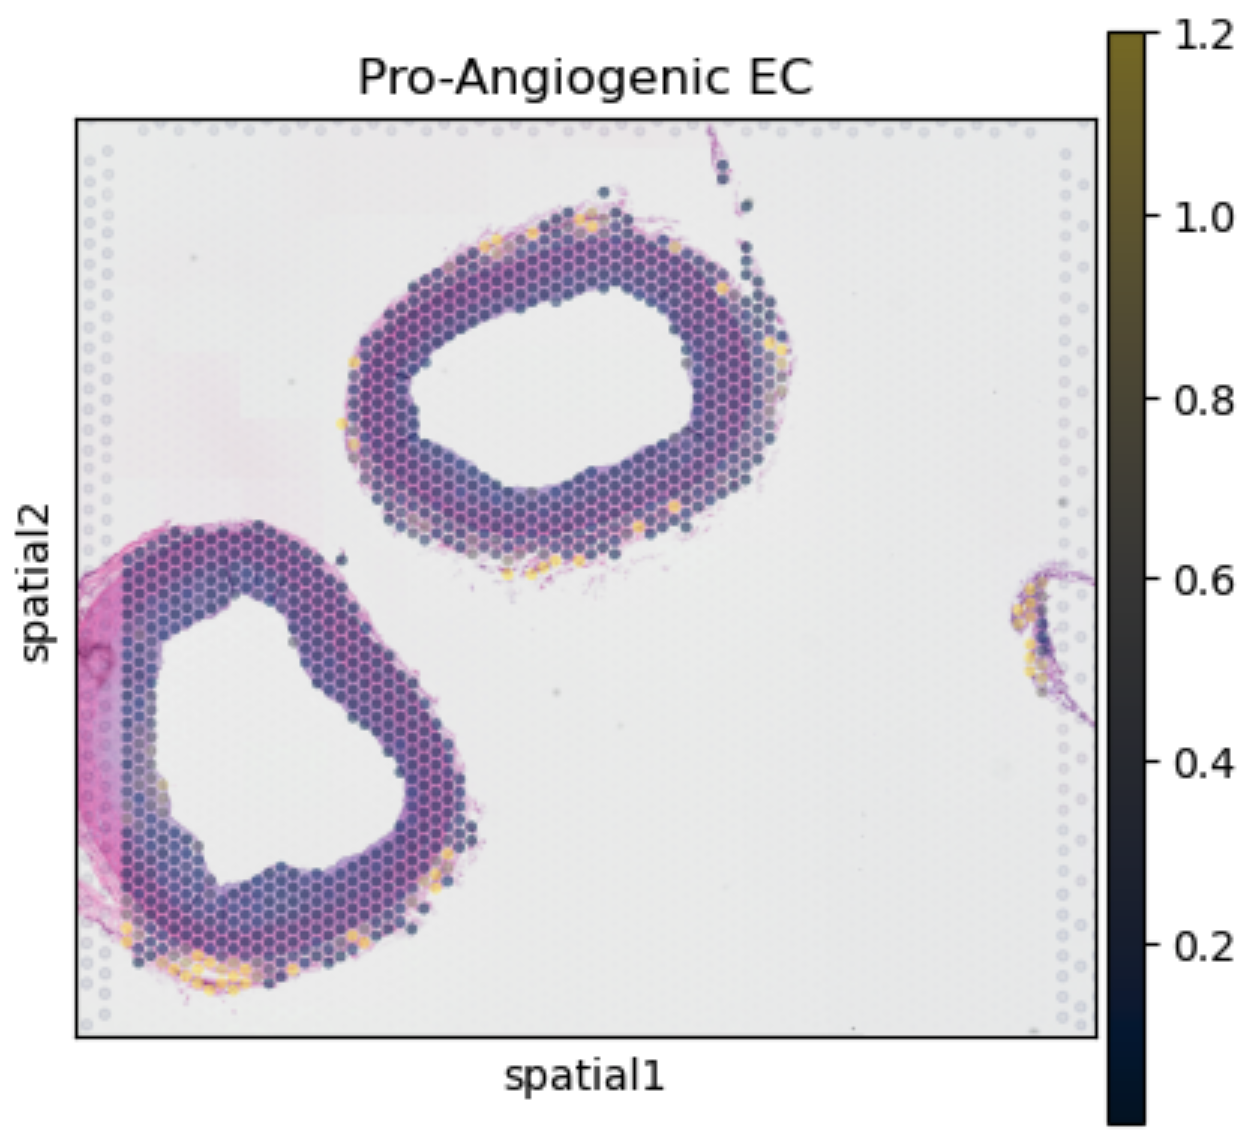
\includegraphics[width=\textwidth]{paecpa11}
\caption{Pro-Angiogenic EC signature in FW106008 intermediate lesion sample}
\label{fig:atherosclerosis_spatial}
\end{subfigure}
\caption{Emerging neovascularization in intermediate lesion sample}
\label{fig:spatial_deconvolution}
\end{figure}

\subsection{Atheromas Display Robust Inflammatory Cell Clusters and Active Neovascularization}
In fully developed atheromas, which showed substantial intimal thickening and necrotic cores, clear signatures of inflammatory and endothelial changes were evident. Pro-angiogenic ECs formed distinct hotspots, particularly along the plaque shoulders and near necrotic areas (Figure 3a), reflecting active microvessel formation. EndoMT ECs became more pronounced, often co-localizing with regions subject to mechanical stress, suggesting a shift toward mesenchymal-like properties that may facilitate extracellular matrix deposition and plaque remodeling. Macrophage populations showed heightened heterogeneity, including foam-cell–like PLIN2\textsuperscript{+}/TREM1\textsuperscript{+} macrophages in lipid-laden zones and HMOX1\textsuperscript{+} macrophages in regions with high oxidative stress (Figure 3b, 2c). Inflammatory macrophages and other subsets interspersed throughout the lesion, frequently bordering localized T-cell clusters. CD4 and CD8 T cells accumulated in sizable aggregates within the plaque shoulders, a pattern consistent with an ongoing immune response that may contribute to further lesion progression or destabilization.
\begin{figure}[H]
\centering
\begin{subfigure}{0.3\textwidth}
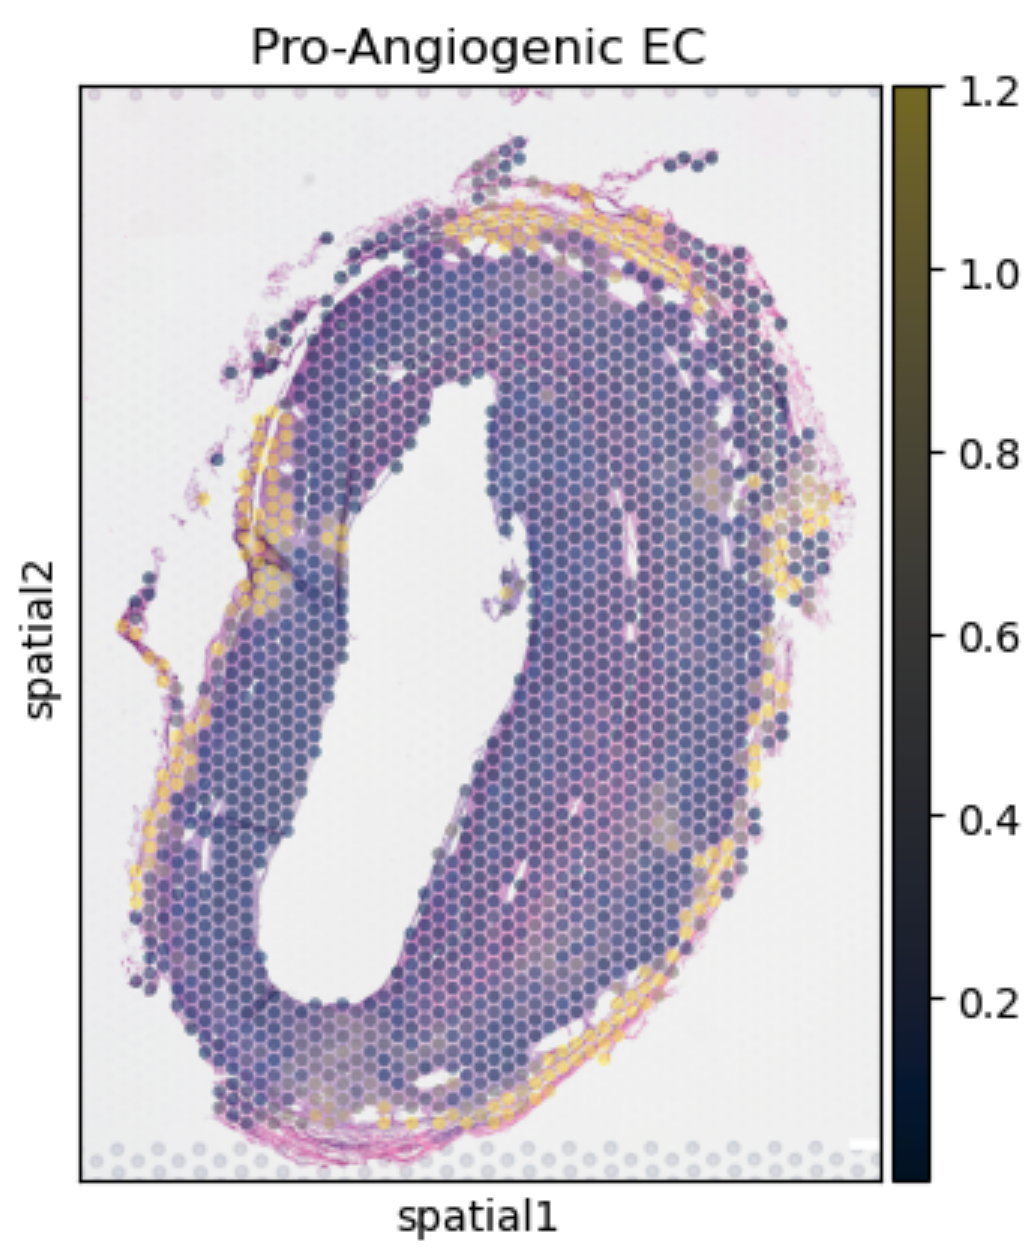
\includegraphics[width=\textwidth]{paecpa4}
\caption{Pro-Angiogenic EC signature}
\label{fig:control_spatial}
\end{subfigure}
\hfill
\begin{subfigure}{0.3\textwidth}
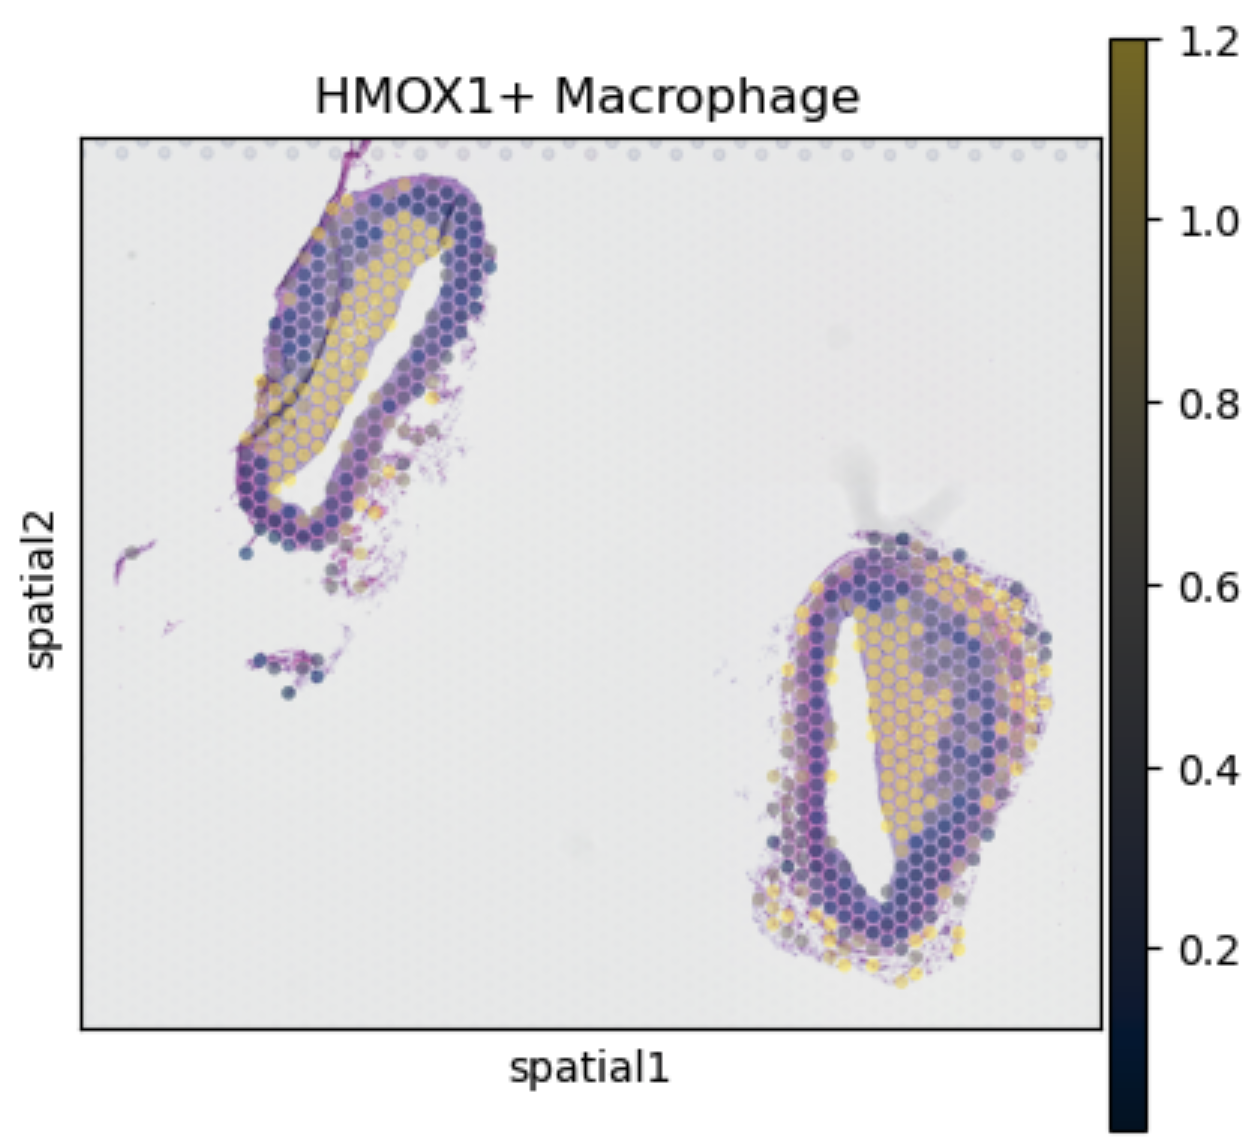
\includegraphics[width=\textwidth]{hmoxpa5}
\caption{HMOX1\textsuperscript{+} macrophage signature}
\label{fig:atherosclerosis_spatial}
\end{subfigure}
\hfill
\begin{subfigure}{0.3\textwidth}
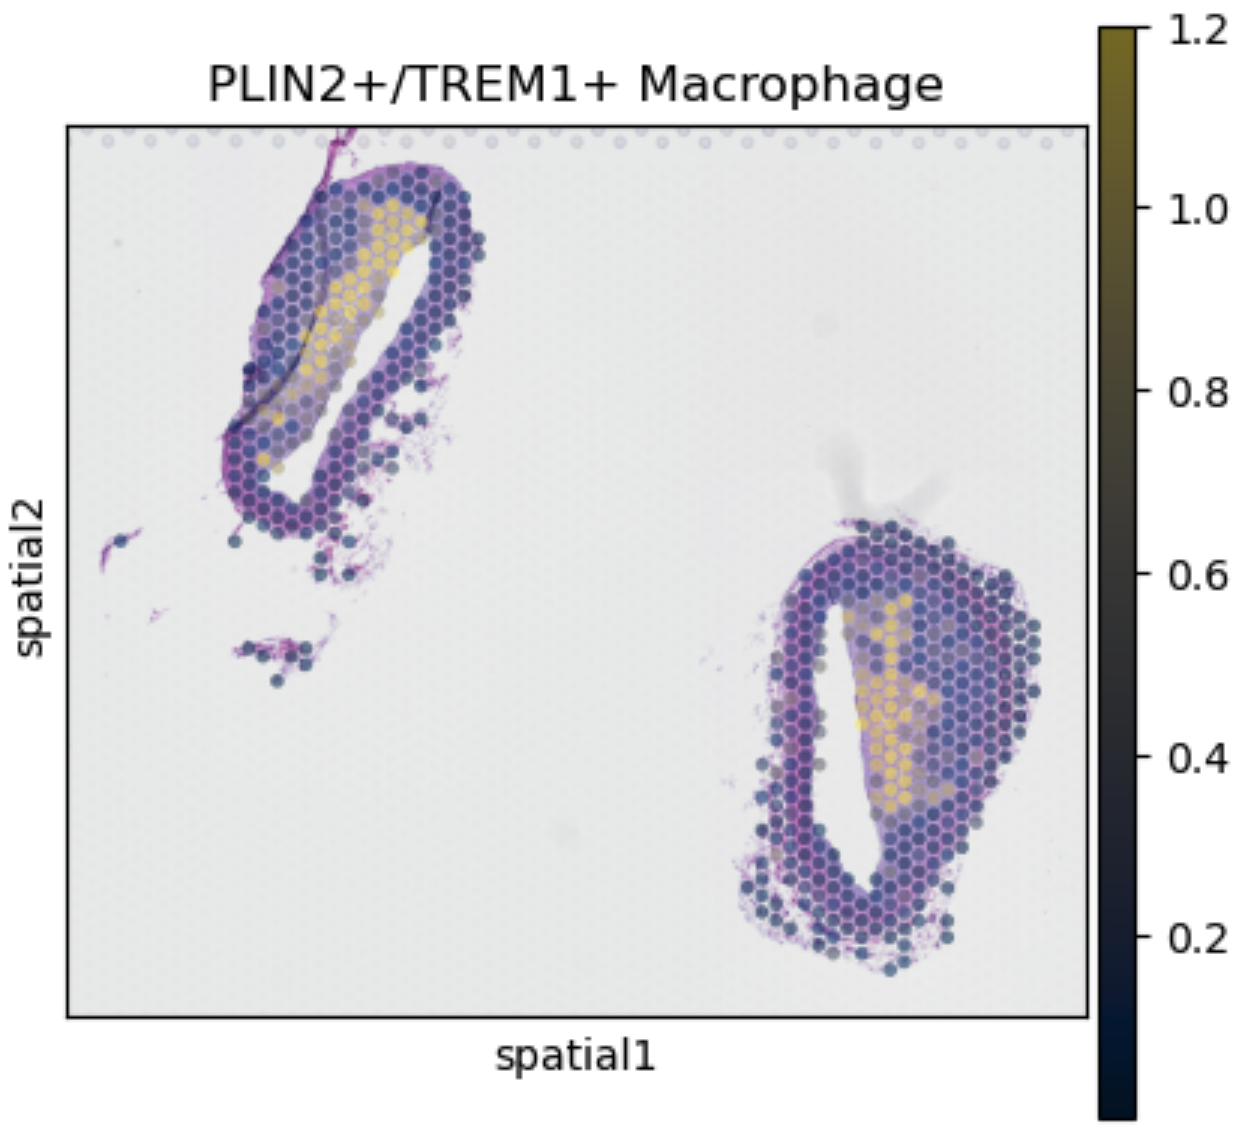
\includegraphics[width=\textwidth]{plnpa6}
\caption{PLIN2\textsuperscript{+}/TREM1\textsuperscript{+} macrophage signature}
\label{fig:atherosclerosis_spatial}
\end{subfigure}
\caption{Inflammatory cell clusters in atheroma samples}
\label{fig:spatial_deconvolution}
\end{figure}
\subsection{Fibroatheromas Exhibit Extensive Lesion Architecture with Thick Fibrous Caps}
In fibroatheromas, an advanced stage of atherosclerosis marked by well-defined fibrous caps overlying large necrotic cores, neovascularization and robust immune infiltrates persisted. Pro-angiogenic ECs (Figure 4a) and EndoMT ECs remained conspicuous along both the fibrous cap and intraplaque microvessels, illustrating the continued plasticity of endothelial populations. Macrophage density was similarly elevated, particularly in zones just beneath the fibrous cap and adjacent to the necrotic core, where oxidative stress and inflammatory cues frequently overlap. Foam-cell–like PLIN2\textsuperscript{+}/TREM1\textsuperscript{+} macrophages indicated prolonged lipid accumulation, while HMOX1\textsuperscript{+} cells provided evidence of sustained oxidative stress (Figure 4b, 3c). Interestingly, both CD4 and CD8 T cells did not exhibit strong presence in the periphery of these macrophage clusters in the plaque shoulder and adventitial areas.
\begin{figure}[H]
\centering
\begin{subfigure}{0.3\textwidth}
\includegraphics[width=\textwidth]{paecpa9}
\caption{Pro-Angiogenic EC signature}
\label{fig:control_spatial}
\end{subfigure}
\hfill
\begin{subfigure}{0.3\textwidth}
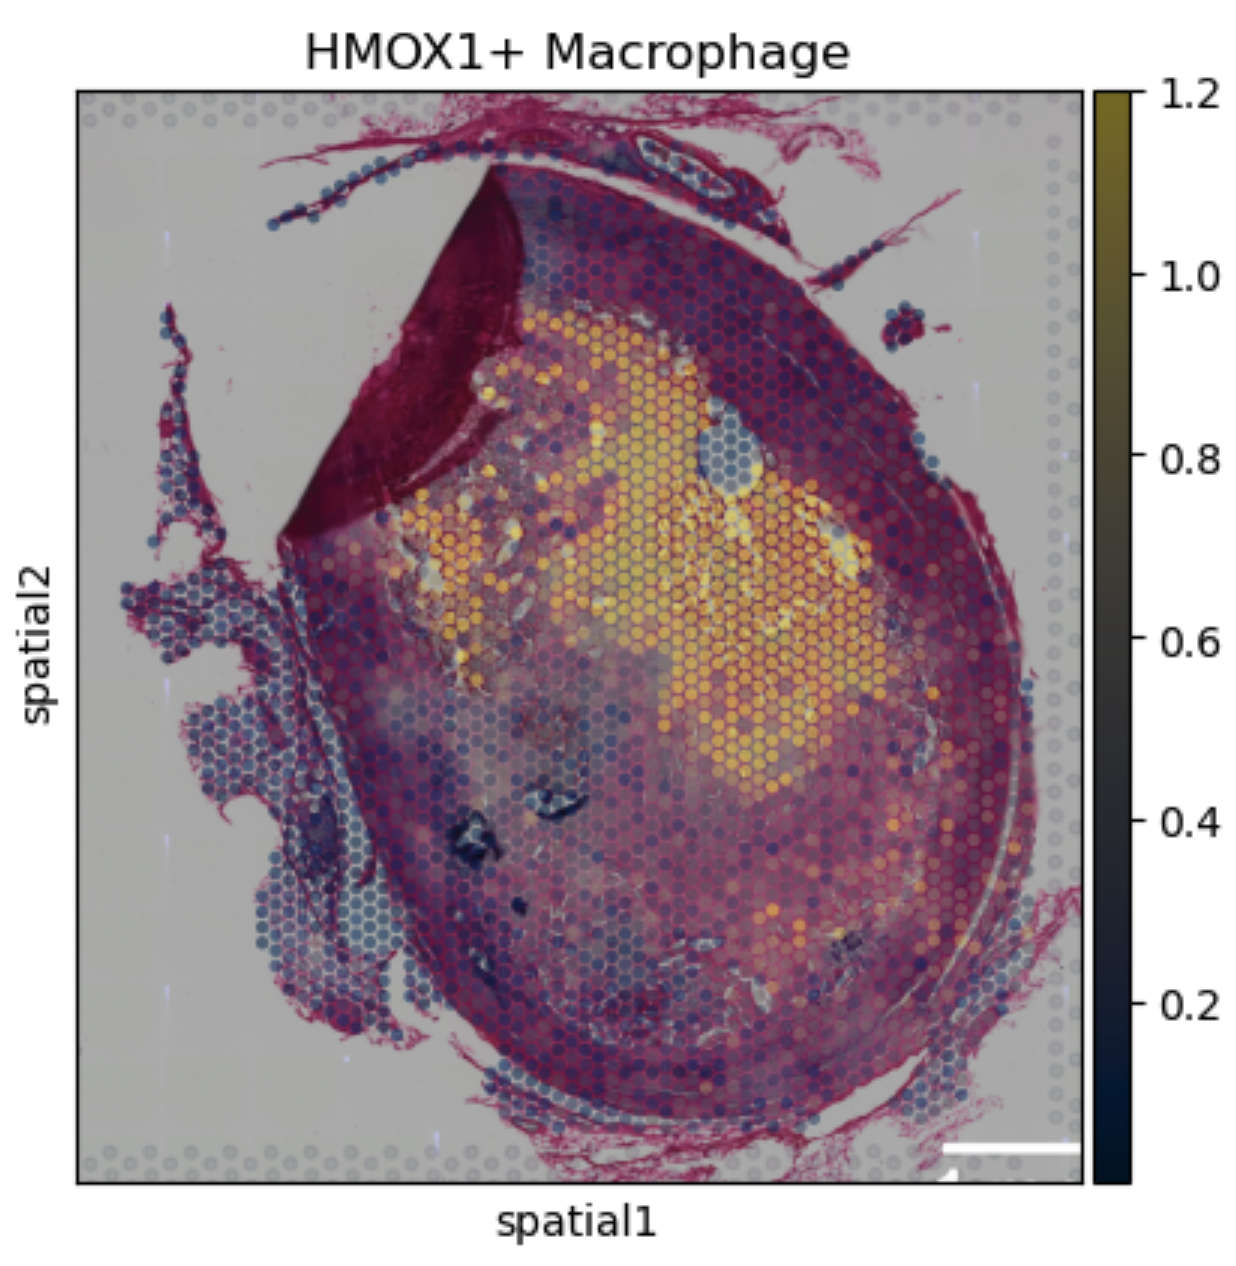
\includegraphics[width=\textwidth]{hmoxpa8}
\caption{HMOX1\textsuperscript{+} macrophage signature}
\label{fig:atherosclerosis_spatial}
\end{subfigure}
\hfill
\begin{subfigure}{0.3\textwidth}
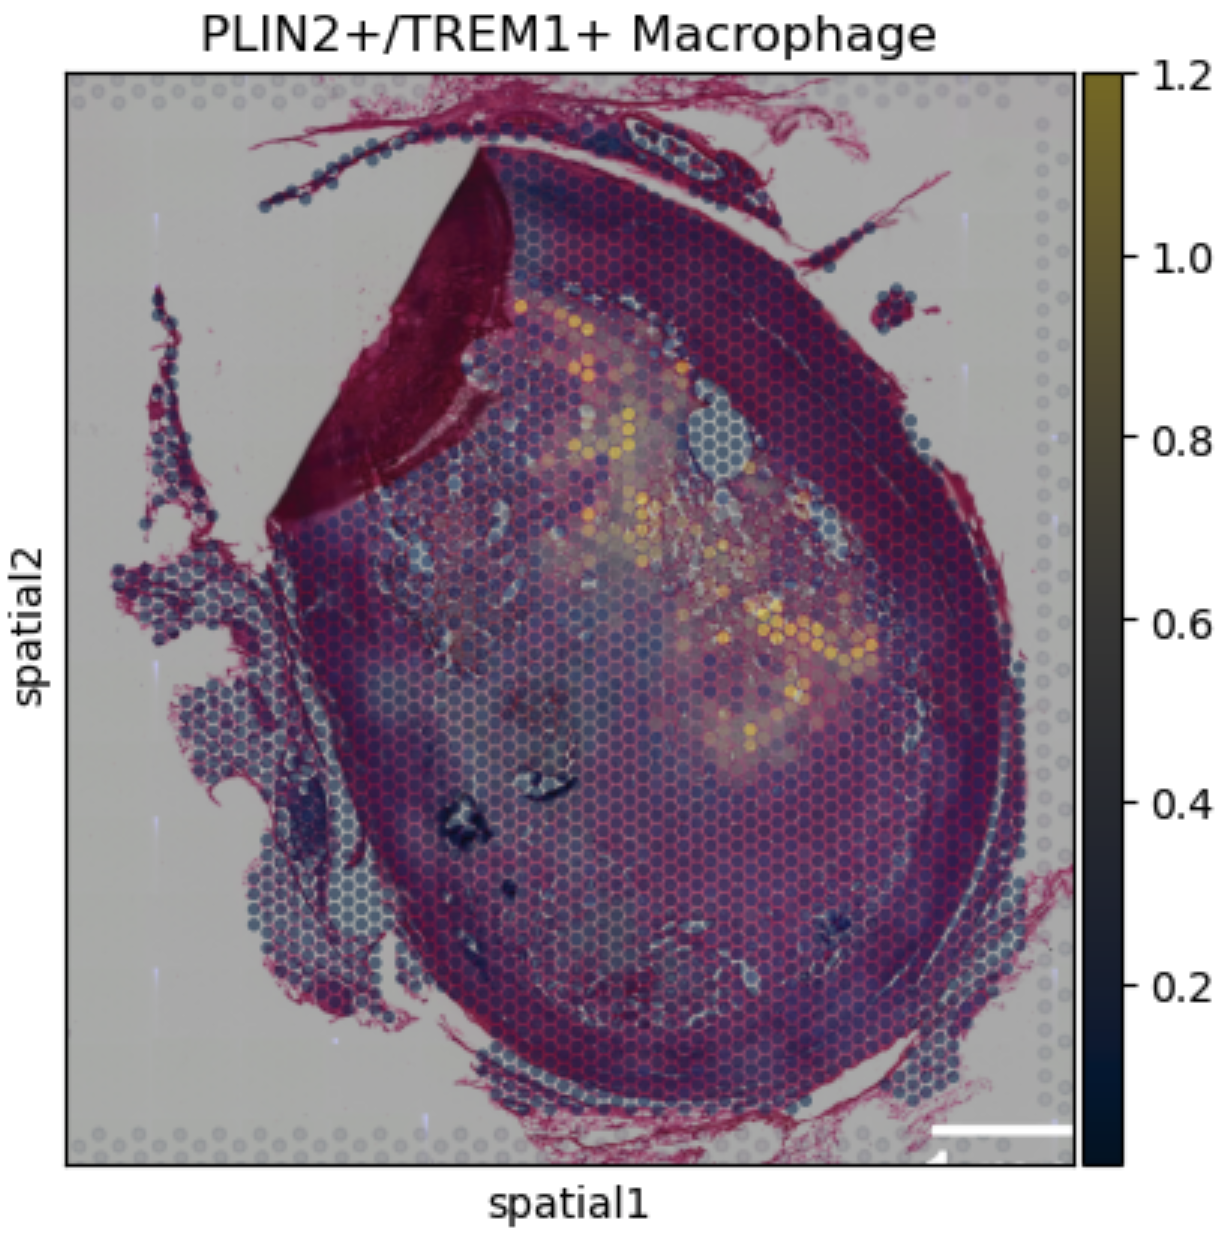
\includegraphics[width=\textwidth]{plnpa7}
\caption{PLIN2\textsuperscript{+}/TREM1\textsuperscript{+} macrophage signature}
\label{fig:atherosclerosis_spatial}
\end{subfigure}
\caption{Inflammatory cell clusters in fibroatheroma samples}
\label{fig:spatial_deconvolution}
\end{figure}
\subsection{Comparative Overview Across Lesion Stages}
Overall, the spatial distribution of immune and endothelial cell types underscores a continuum of disease progression from minimal immune activation and quiescent endothelium in control vessels to intensely inflamed and highly vascularized tissue in fibroatheromas. Early lesions are typified by modest neovascular sprouts and low to moderate immune cell clustering, whereas atheromas show more pervasive endothelial remodeling and heterogenous macrophage populations, often in proximity to T-cell aggregates. Fibroatheromas extend these patterns, featuring thick fibrous caps, necrotic cores, persistent oxidative stress, and active neovascularization. Pro-angiogenic ECs consistently expanded across the plaque stages, correlating with increasing neovascular niches, while EndoMT ECs became more evident in advanced disease, hinting at endothelial cells acquiring mesenchymal traits that may facilitate further matrix deposition. Together, these findings reveal that progressive endothelial plasticity and macrophage/T-cell crosstalk shape the complex microenvironment of the atherosclerotic plaque, illuminating key processes that could be therapeutically targeted to modulate plaque growth and stability.

\subsection{}
Was auch noch cool wäre ist wenn ihr die ergebnisse der spatial deconvolution mit den bulk deconvolution ergebnissen in meinem preprint vergleicht (Figure 6). wir haben auch den unterschied in HMOX1 macrophagen zwischen early und late lesions in carotid arteries gesehen.


\subsection{Spatial Mapping of Endothelial Cell Subtypes}
Pro-angiogenic ECs were predominantly localized within neovascularized regions of the plaque.

\begin{itemize}
  \item Visualization of EC distribution in atherosclerotic plaques.
  \item Quantification of pro-angiogenic EC abundance across spatial zones.
\end{itemize}

\subsection{Co-localization with Other Cell Types}
These cells were frequently found near macrophages and smooth muscle cells, indicating potential interactions in plaque progression.

\begin{itemize}
  \item Interaction with macrophages, smooth muscle cells, and fibroblasts.
  \item Presence in adventitia vs. neointima.
\end{itemize}

\subsection{Gene Expression and Pathway Analysis}
Differential expression analysis revealed key angiogenic pathways, including VEGF signaling and extracellular matrix remodeling.

\begin{itemize}
  \item Differential expression analysis between pro-angiogenic ECs and other EC subsets.
  \item Enriched pathways related to angiogenesis and plaque progression.
\end{itemize}

\subsection{Comparison of deconvolution results with Sikander Hayat deconvolution}
Comparison of deconvolution results with Sikander Hayat deconvolution.

Our spatial deconvolution results align with key observations reported in previous studies of atherosclerotic plaque composition and vascular remodeling \citep{Bleckwehl2025-td}. Specifically, it has been noted that fibroblasts are primarily located in the outer layers of the arterial wall, especially within the adventitia, whereas immune cells adopt a bimodal distribution, populating both the adventitial region and the inner arterial wall. In our dataset, we similarly observed a higher relative abundance of fibroblast-like cells at the periphery of the tissue sections, in agreement with the notion that they accumulate in regions of dense extracellular matrix and perivascular remodeling. 

Likewise, the increased accumulation of immune cells in advanced lesions reported by earlier work parallels our own findings, which showed greater infiltration of various macrophage phenotypes and T cells near both the luminal side and the adventitial boundary of atherosclerotic plaques. This bimodal immune presence appears to intensify with disease severity, emphasizing a coordinated inflammatory response that extends beyond superficial plaque regions and involves the deeper layers of the vessel wall.

Furthermore, previous research distinguished two endothelial cell clusters—one enriched in the adventitia and another localizing primarily to the luminal endothelium—based on characteristic gene expression profiles (e.g., venular vs. arterial signatures). In our analysis, pro-angiogenic endothelial cells were found predominantly near neovascularized plaque regions and showed spatial overlap with inflammatory hotspots, while EndoMT endothelial cells were enriched in structurally stressed or fibrous areas. Although our findings highlight distinctive states of endothelial plasticity rather than strictly venular or arterial subtypes, these results are broadly consistent with the idea that endothelial cell populations may segregate according to the local microenvironmental conditions in the plaque (e.g., hypoxia, shear stress, and cytokine milieu). Markers shared by both endothelial subtypes, such as VWF, also corresponded to regions of robust endothelial presence in our spatial maps, similar to the dual distribution pattern noted in previous reports.

Taken together, these parallels reinforce the concept that atherosclerosis involves dynamic changes in both vascular and stromal cell populations, manifesting as gradients of fibroblasts, immune cells, and distinct endothelial cell phenotypes across the arterial wall. By integrating single-cell references with spatial transcriptomics, we add further resolution to these processes, clarifying how angiogenic and mesenchymal-like endothelial populations interface with immune cells and fibroblasts in different plaque compartments. Our results thus corroborate and extend prior evidence for compartment-specific cell distributions, shedding light on how these diverse populations shape and maintain the atherosclerotic microenvironment.




\section{Discussion}

\subsection{Biological Implications}
The spatial deconvolution presented in this study highlights the critical role of pro-angiogenic endothelial cells (ECs) in the development and progression of atherosclerotic plaques. By localizing predominantly within neovascularized regions of lesions, these cells likely contribute to the formation of intraplaque microvessels that can fuel local inflammation and facilitate continued plaque growth. The observed co-localization of pro-angiogenic ECs with macrophage- and smooth muscle cell–rich areas suggests bidirectional interactions, wherein endothelial cells contribute to angiogenesis and vessel permeability while inflammatory cells provide cytokines and growth factors that further stimulate neovascularization. This positive feedback loop may predispose plaques to instability and rupture, implicating pro-angiogenic ECs in the transition from stable fibrotic lesions to high-risk phenotypes.

Although the neovascular networks developed by pro-angiogenic ECs can enhance oxygen and nutrient supply to growing plaques, they may also exacerbate tissue damage by increasing leukocyte infiltration and oxidative stress within the lesion microenvironment. Moreover, the enrichment of EndoMT (Endothelial-to-Mesenchymal Transition) ECs in more advanced plaques implies that endothelial cells undergo phenotypic changes conducive to extracellular matrix remodeling. Taken together, these findings raise the possibility that targeting specific endothelial subpopulations and their signaling pathways could represent a therapeutic strategy to limit disease progression and improve plaque stability.

\subsection{Methodological Considerations}
The combination of high-throughput spatial transcriptomic data and single-cell reference atlases offers a powerful means to unravel the cellular landscape of complex tissues. By applying Cell2Location \citep{Kleshchevnikov2022-vd}, we were able to identify and quantify rare and functionally important subsets, such as pro-angiogenic and EndoMT ECs, across thousands of spatial spots. This Bayesian framework can robustly account for technical variability between experiments and produce absolute abundance estimates, thus overcoming some of the limitations inherent to more conventional deconvolution methods.

However, several considerations remain crucial. First, accurate inference depends on the representativeness of the single-cell reference dataset. If certain cell subtypes are undersampled or misannotated in the scRNA-seq reference, downstream spatial deconvolution may be biased or incomplete. Second, the resolution of Visium spots precludes single-cell level mapping, and each spot typically encompasses multiple cell types. While Cell2Location partly addresses this by leveraging probabilistic modeling, complementary validation at the protein level (e.g., through immunohistochemistry or spatial proteomics) is needed to confirm localized cell-type identities and states. Finally, comparison with alternative deconvolution algorithms—such as RCTD or SPOTlight—can provide additional cross-validation and highlight method-specific strengths or limitations. Combining these approaches may yield a more comprehensive picture of the spatial architecture of the atherosclerotic plaque.

\subsection{Future Directions}
Future investigations should build on these findings by integrating additional omics modalities to capture the multi-faceted nature of the plaque microenvironment. Spatial proteomic or spatial metabolomic analyses could validate and refine the putative cell-cell interactions revealed here, adding mechanistic depth to transcriptional signatures. Moreover, live-imaging or lineage-tracing approaches could help delineate the temporal dynamics of pro-angiogenic and EndoMT endothelial cells, clarifying whether and how they transition between states during plaque development.

Beyond the integration of multi-omics, a key priority is translating these spatial insights into functional models. Experimentally manipulating the specific signaling pathways driving pro-angiogenic EC expansion or EndoMT activation in vivo or in vitro may elucidate novel targets for therapeutic intervention. Given the heterogeneity of atherosclerosis across vascular beds and between individuals, future studies should also encompass larger patient cohorts and multiple arterial territories to define conserved versus context-specific endothelial behaviors. Collectively, these steps will help to transform the detailed spatial maps of cell populations into clinically actionable strategies for personalized management of atherosclerosis.

Bezüglich eurem kommentar in future directions. vor ein par tagen kam ein preprint raus (https://www.medrxiv.org/content/10.1101/2025.02.09.25321955v1) der sich spatial proteomics auf coronary arteries angeschaut hat. Vlt haben die auch irgendwelche interestanten ergebnisse die mit unseren überlappen... Falls ihr die Zeit dafür findet wäre das noch ein bonus. Sind aber auch jetzt schon wirklich super ergebnisse!
\begin{comment}
\subsection{Biological Implications}
Our findings suggest that pro-angiogenic ECs contribute to neovascularization and may play a role in plaque instability.

\begin{itemize}
  \item Role of pro-angiogenic ECs in vascular remodeling and plaque instability.
  \item Potential implications for therapeutic targeting.
\end{itemize}

\subsection{Methodological Considerations}
While Cell2Location provides high-resolution spatial deconvolution, validation through experimental methods such as spatial proteomics is necessary.

\begin{itemize}
  \item Strengths and limitations of Cell2Location for spatial deconvolution.
  \item Comparison with alternative deconvolution methods.
\end{itemize}

\subsection{Future Directions}
Further studies integrating multi-omics data could enhance our understanding of endothelial heterogeneity in atherosclerosis.

\begin{itemize}
  \item Need for validation using experimental methods (e.g., spatial proteomics).
  \item Potential for integrating multi-omics data (e.g., spatial metabolomics).
\end{itemize}

\end{comment}

\section{Conclusion}
This study maps the spatial distribution of pro-angiogenic ECs in atherosclerotic plaques, providing insights into their role in vascular remodeling and plaque progression.

This work demonstrates that combining single-cell reference atlases with spatial transcriptomics via Cell2Location enables a refined delineation of endothelial cell heterogeneity in human atherosclerotic plaques. We reveal that pro-angiogenic ECs are not only present in mature lesions but also exhibit distinct spatial clustering near inflammatory cells, thereby implicating them in both disease progression and the potential for plaque destabilization. These findings highlight the critical role of endothelial specialization in orchestrating vascular remodeling and immune responses within plaque microenvironments.

By offering high-resolution maps of cellular interactions, spatial transcriptomics paves the way for new hypotheses regarding the molecular drivers of plaque growth and rupture risk. Future studies targeting the biology of pro-angiogenic and EndoMT endothelial cells may hold promise for therapeutic interventions aimed at stabilizing or regressing atherosclerotic lesions. In this context, the integration of additional omics layers, along with validation in diverse patient cohorts, is poised to deepen our understanding of endothelial biology and to advance precision medicine approaches for cardiovascular diseases.

\begin{itemize}
  \item Summary of findings and their relevance to atherosclerosis research.
  \item Final remarks on the significance of spatial transcriptomics for understanding vascular biology.
\end{itemize}


\bibliographystyle{apalike}
\bibliography{references}  % Ensure you have a references.bib file

\newpage
\appendix
\section{Appendix: Data availability}  
Detailed information on the data used for this study can be found in the Methods. Information about the Visium data used for this study can be found at \url{https://zenodo.org/records/14007461} and \url{https://www.10xgenomics.com/products/spatial-gene-expression}, respectively. All other remaining data are available within the article or may be available from the authors upon request.  

\section{Appendix: Code availability}  
The code for this study is available on GitHub at \url{https://github.com/github4touchdouble/proangioec_cell2location_visium}. 

\section{Appendix: Additional Figures}
\begin{figure}[h]
    \centering
    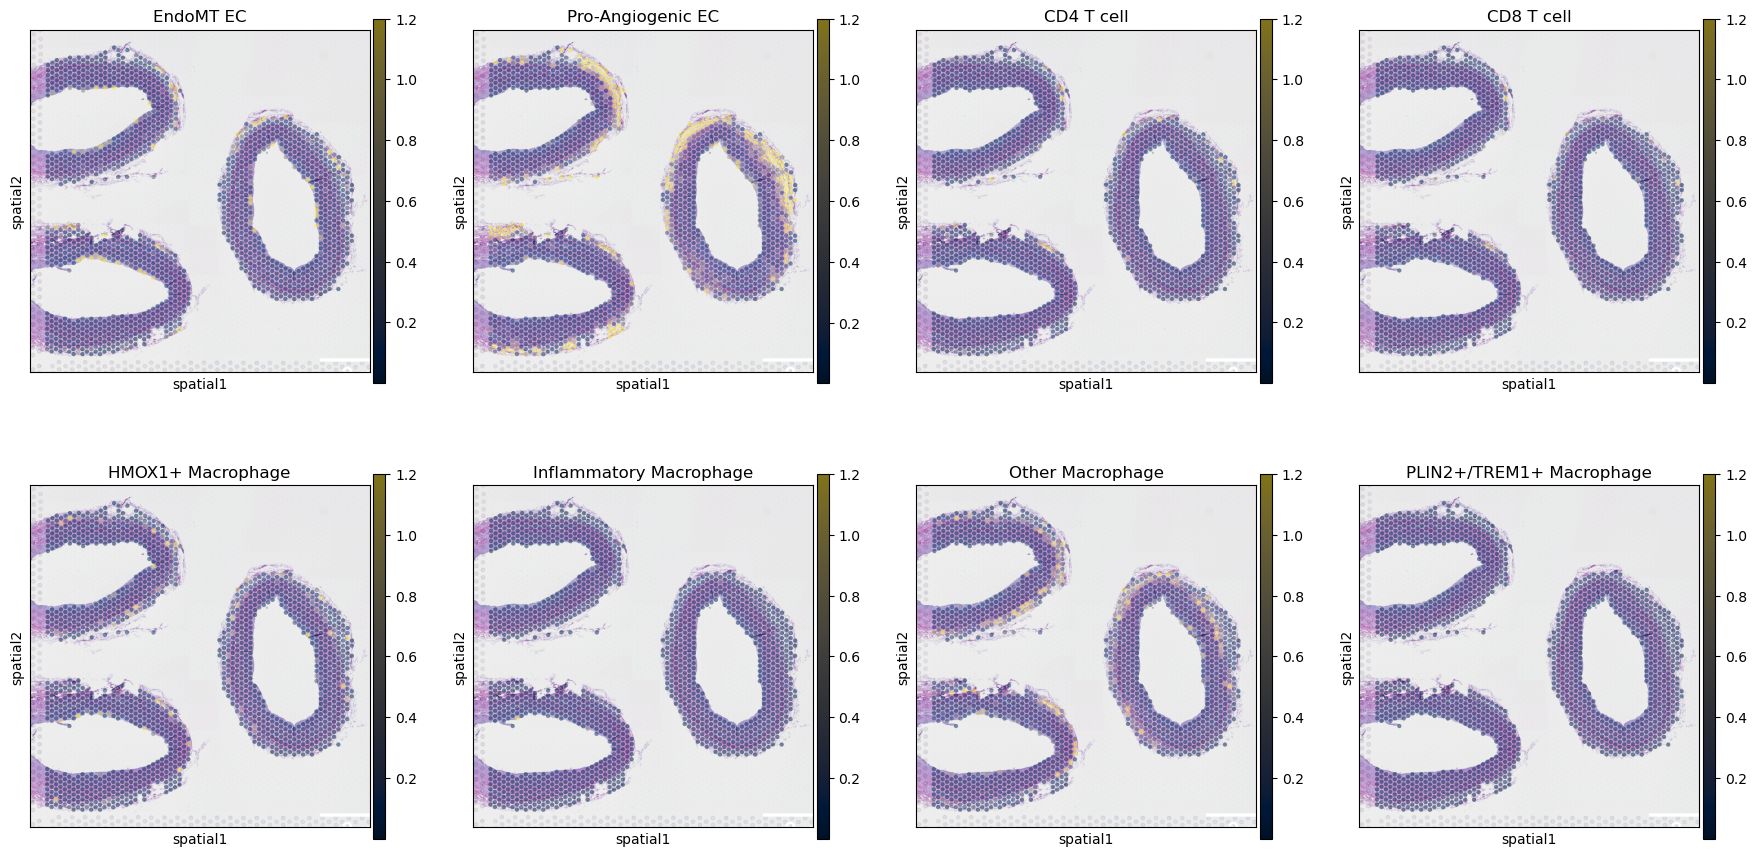
\includegraphics[width=1.1\textwidth]{spatialControl1}
    \caption{Spatial cell types for control sample FW106012}
    \label{fig:appendix1}
\end{figure}
\begin{figure}[h]
    \centering
    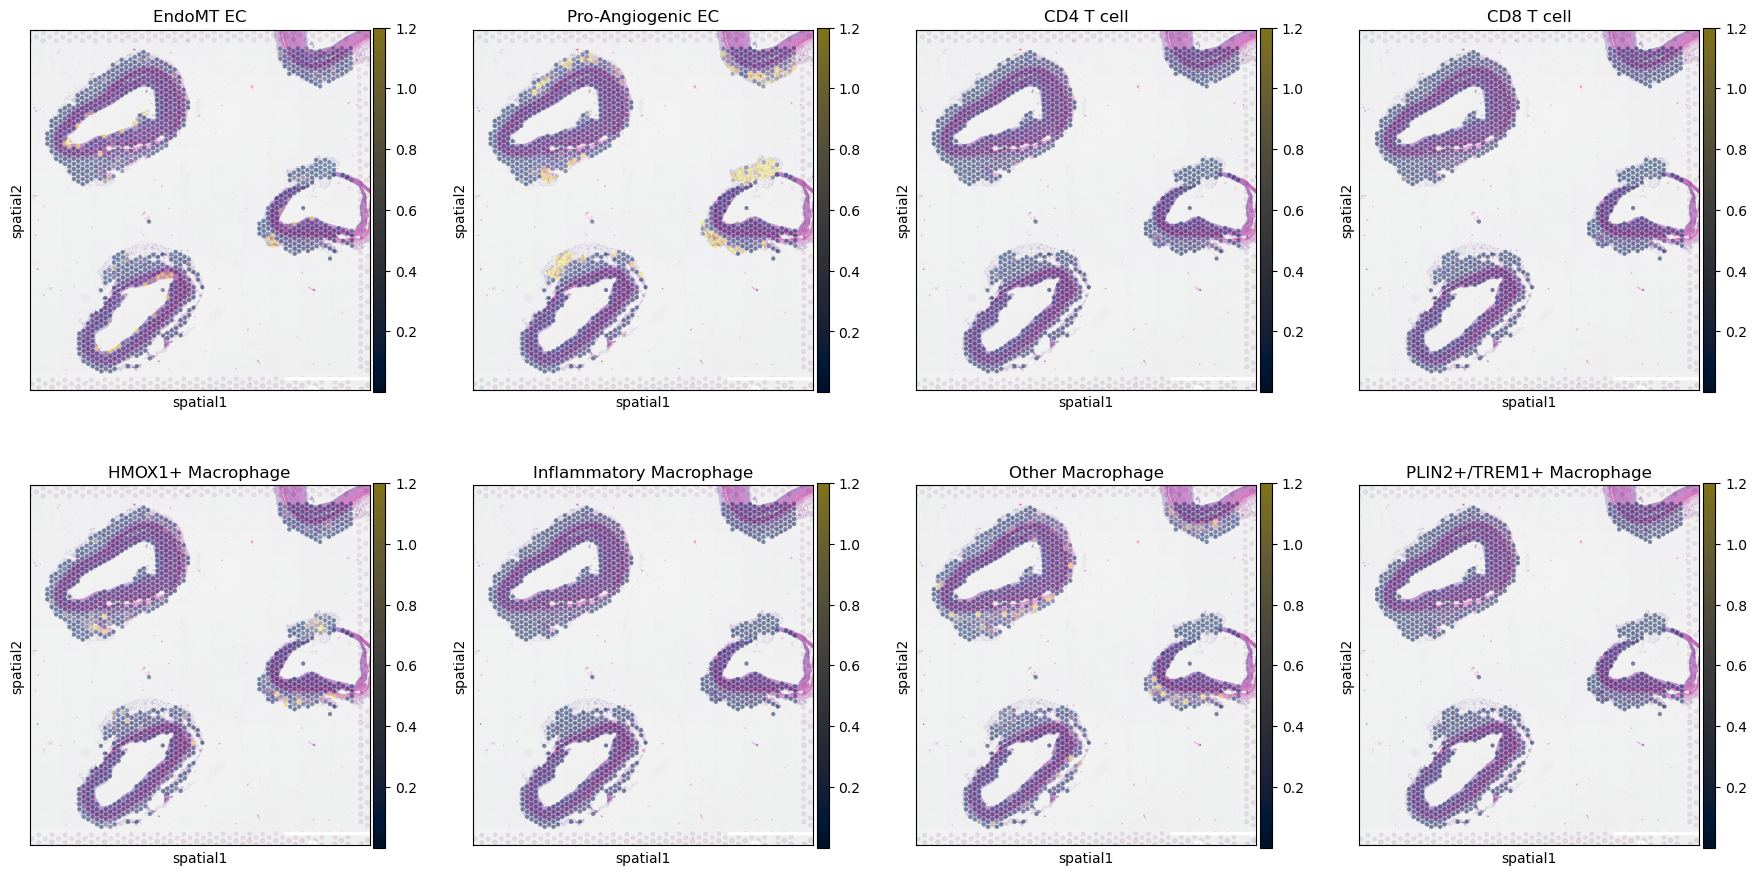
\includegraphics[width=1.1\textwidth]{spatialControl2}
    \caption{Spatial cell types for control sample FW106010}
    \label{fig:appendix1}
\end{figure}
\begin{figure}[h]
    \centering
    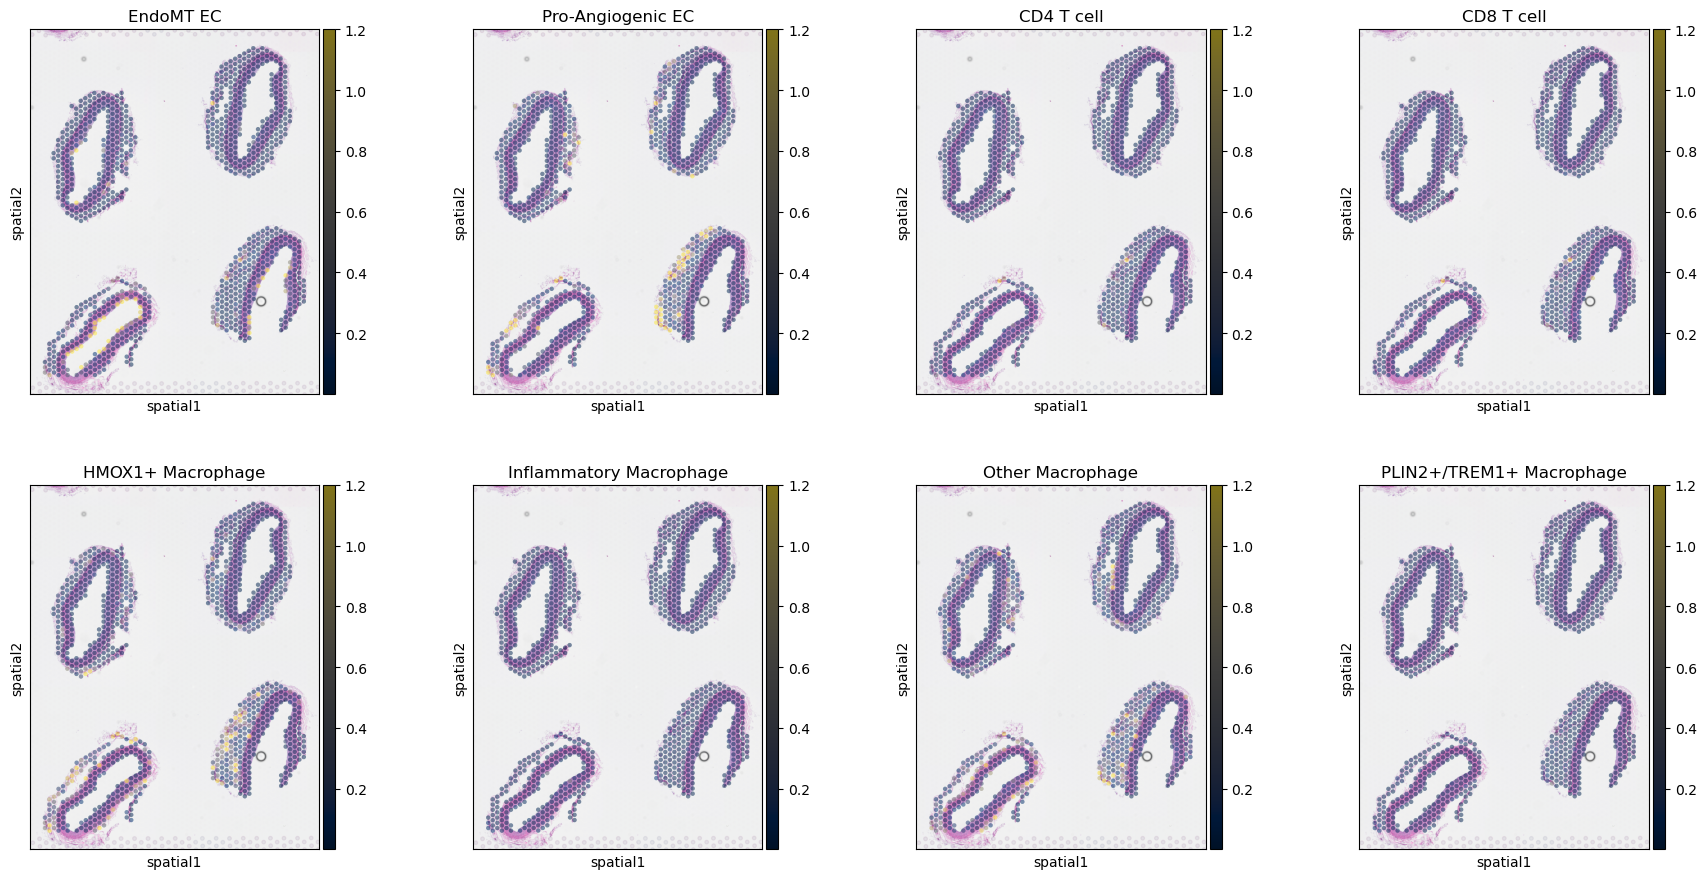
\includegraphics[width=1.1\textwidth]{spatialControl3}
    \caption{Spatial cell types for control sample FW106018}
    \label{fig:appendix1}
\end{figure}
\begin{figure}[h]
    \centering
    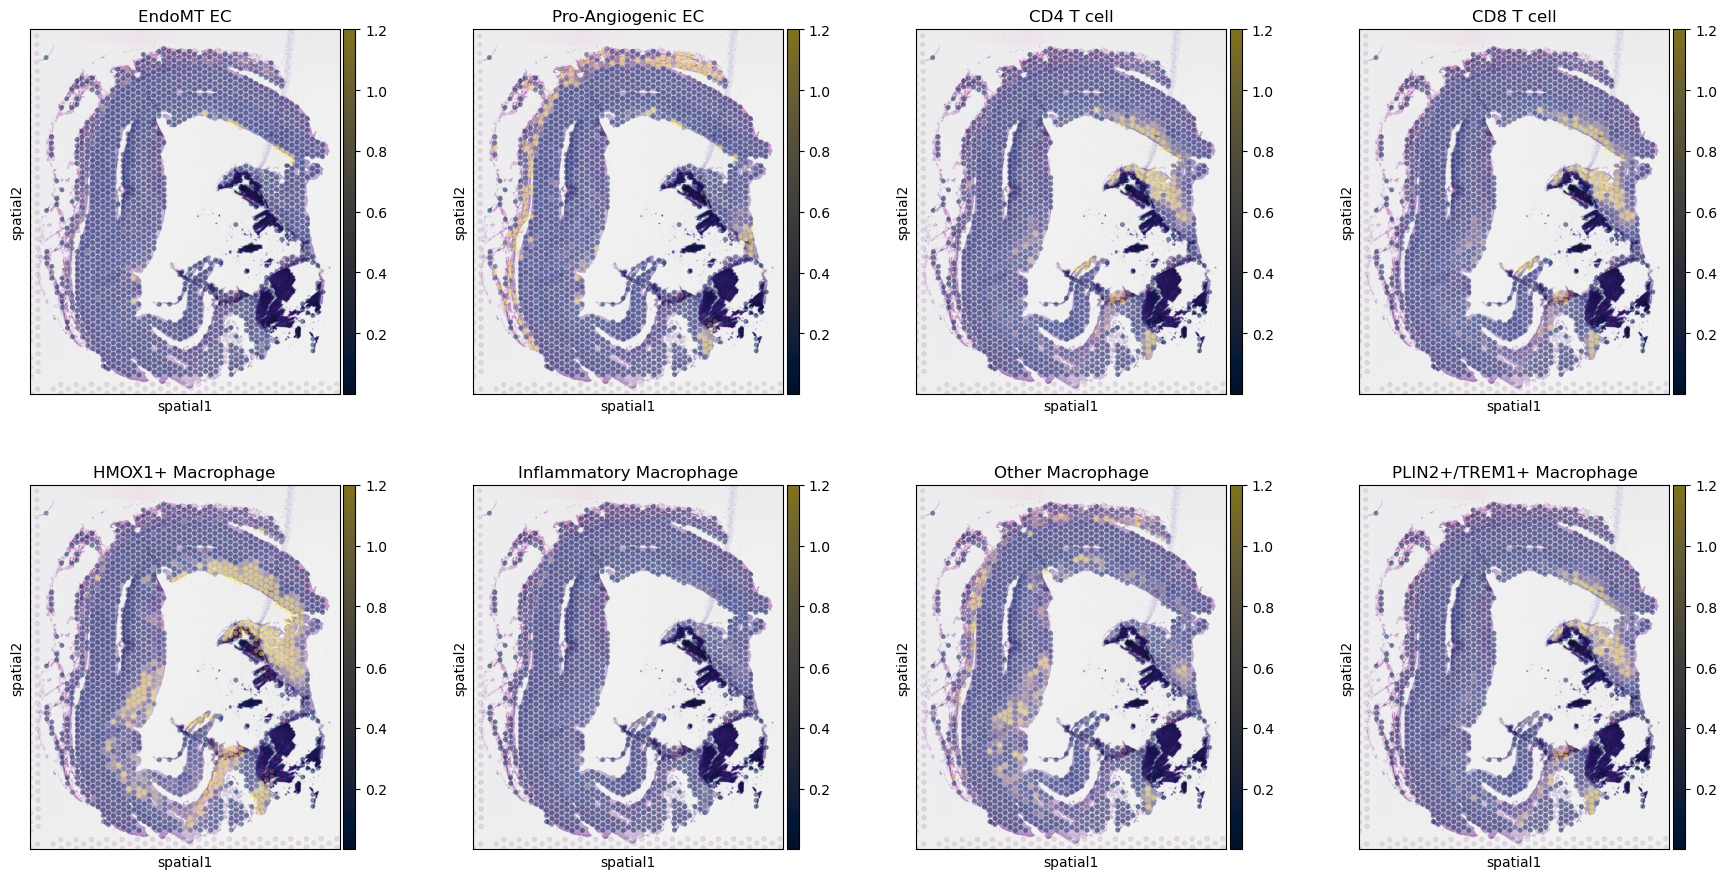
\includegraphics[width=1.1\textwidth]{spatialAtheroma1}
    \caption{Spatial cell types for atheroma sample FW106022}
    \label{fig:appendix1}
\end{figure}
\begin{figure}[h]
    \centering
    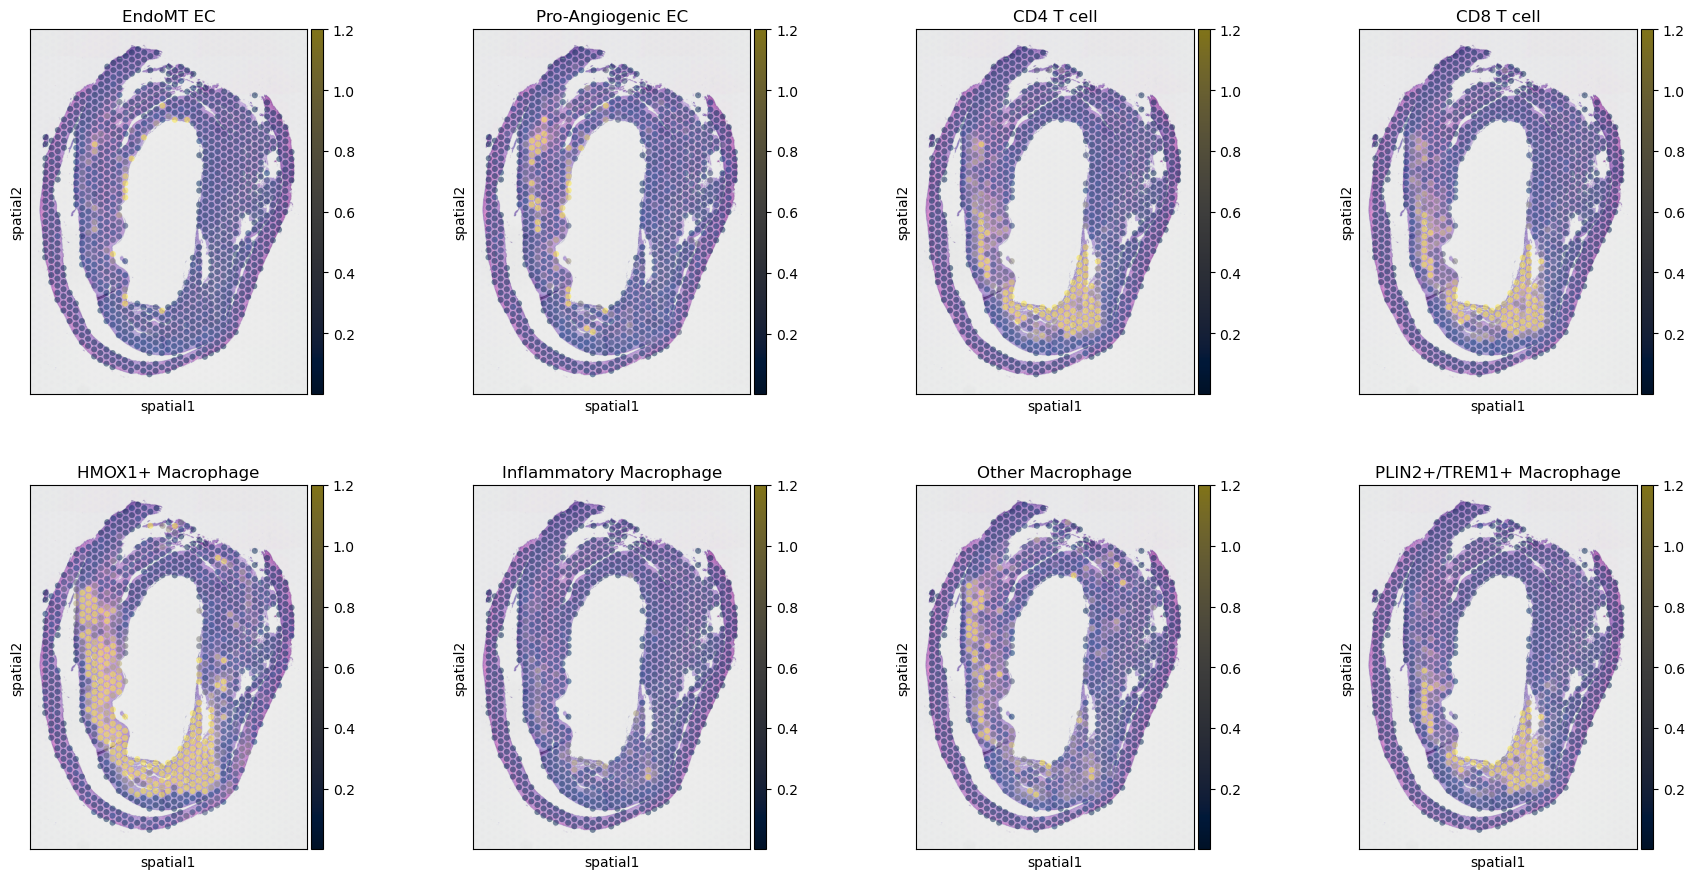
\includegraphics[width=1.1\textwidth]{spatialAtheroma2}
    \caption{Spatial cell types for atheroma sample FW104860}
    \label{fig:appendix1}
\end{figure}
\begin{figure}[h]
    \centering
    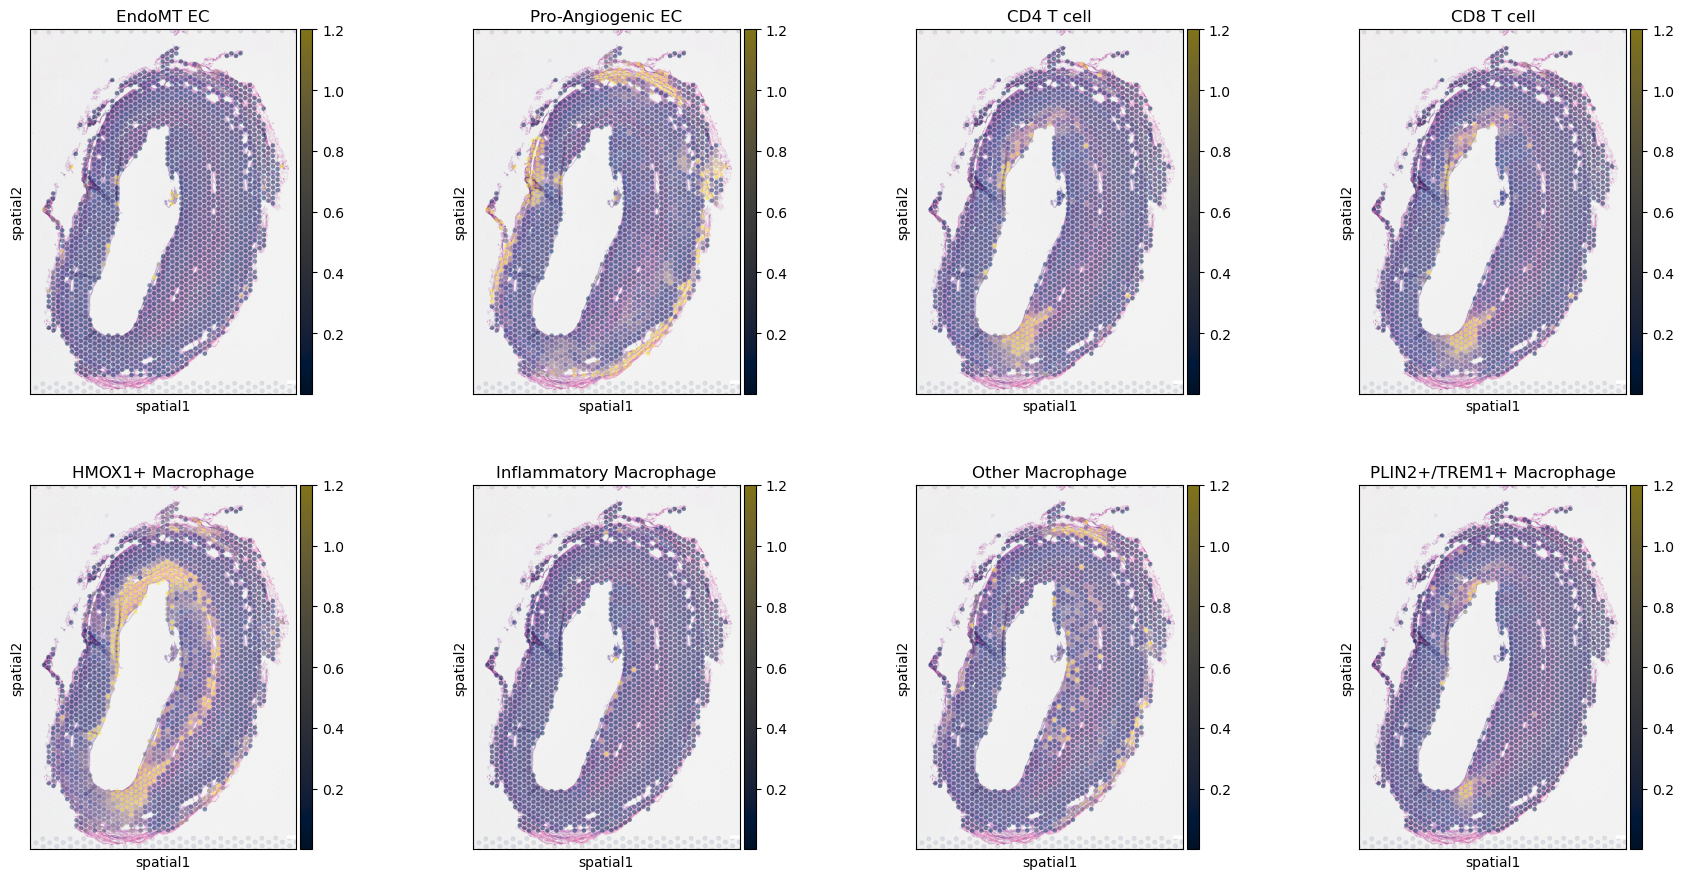
\includegraphics[width=1.1\textwidth]{spatialAtheroma3}
    \caption{Spatial cell types for atheroma sample FW106005v2}
    \label{fig:appendix1}
\end{figure}
\begin{figure}[h]
    \centering
    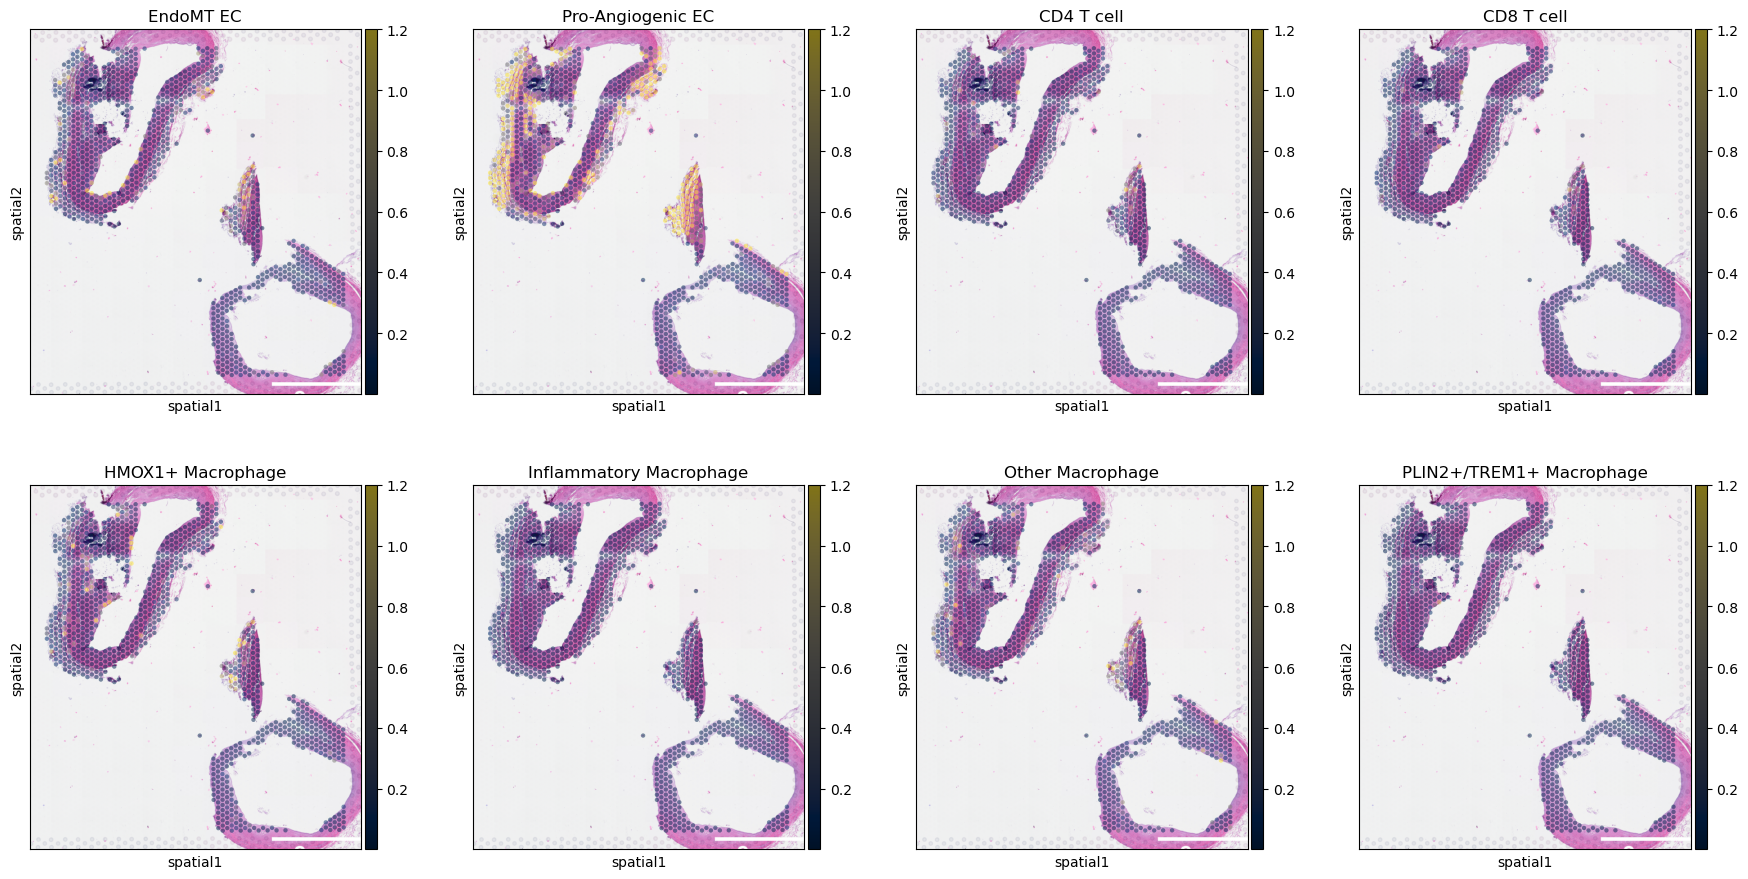
\includegraphics[width=1.1\textwidth]{spatialAtheroma4}
    \caption{Spatial cell types for atheroma sample FW106014}
    \label{fig:appendix1}
\end{figure}
\begin{figure}[h]
    \centering
    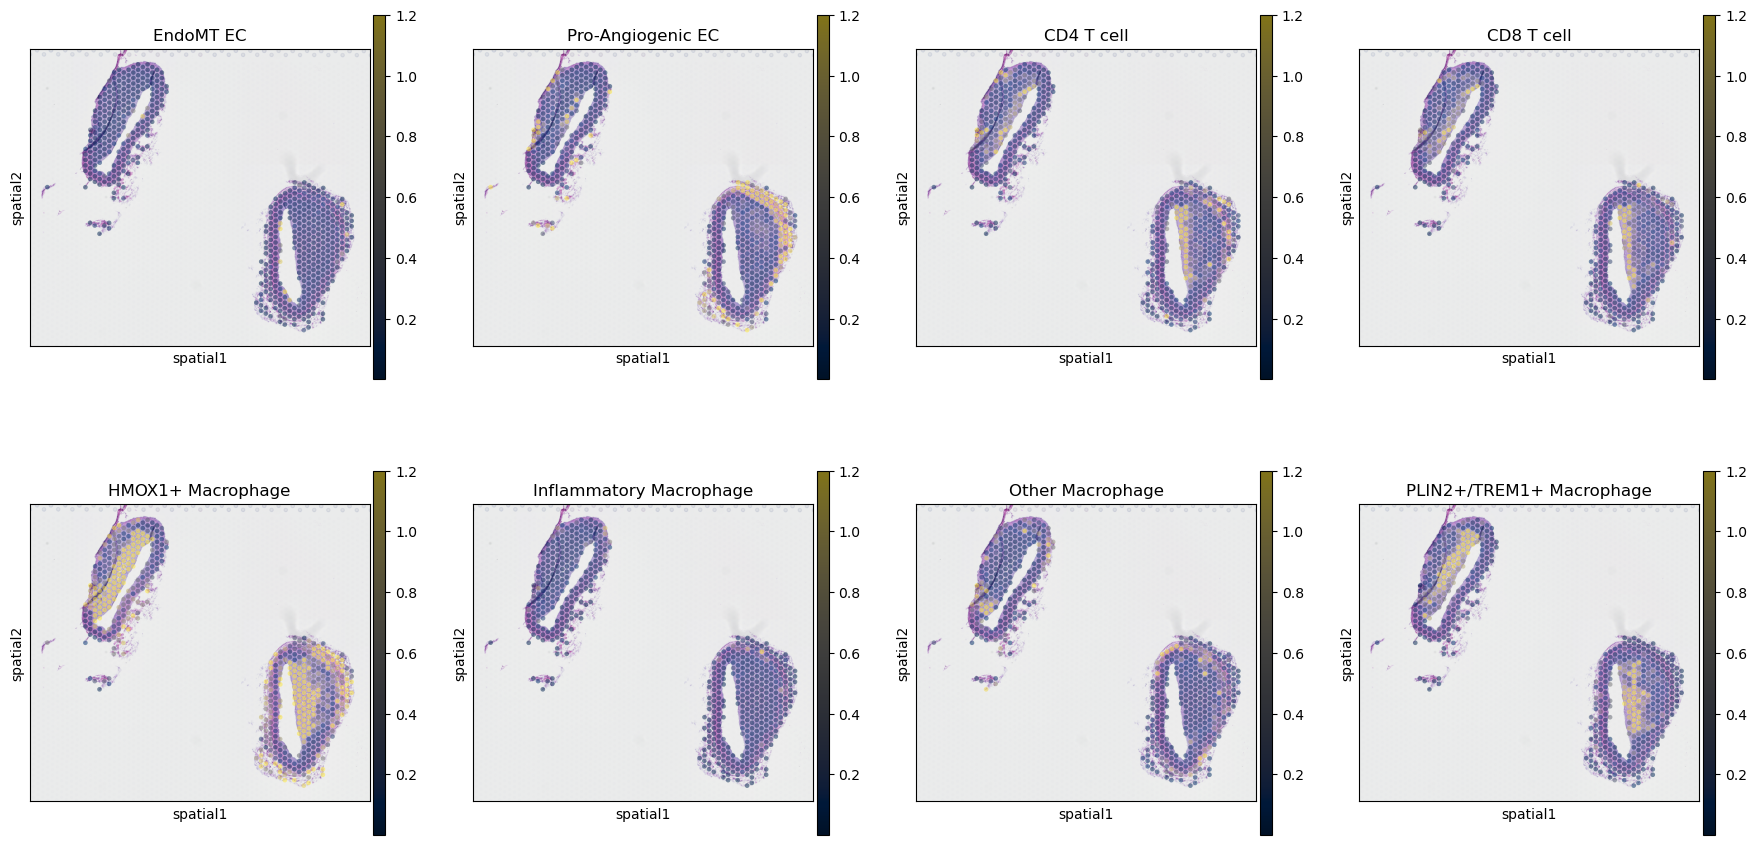
\includegraphics[width=1.1\textwidth]{spatialAtheroma5}
    \caption{Spatial cell types for atheroma sample FW106016}
    \label{fig:appendix1}
\end{figure}
\begin{figure}[h]
    \centering
    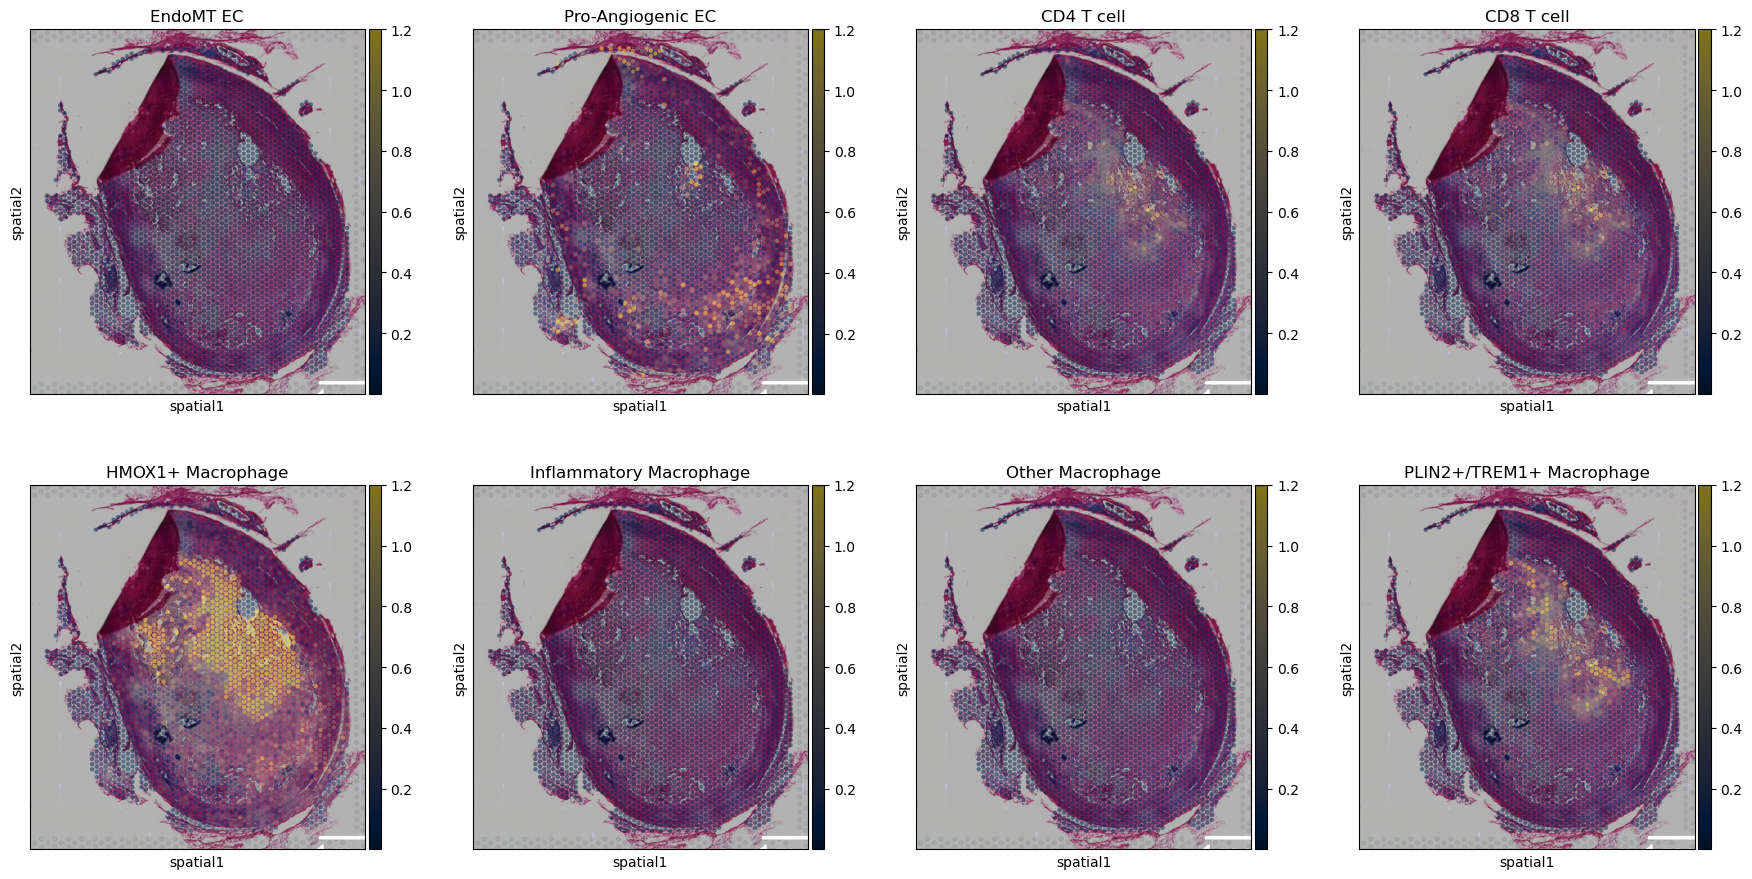
\includegraphics[width=1.1\textwidth]{spatialFibroatheroma1}
    \caption{Spatial cell types for fibroatheroma sample FW104302}
    \label{fig:appendix1}
\end{figure}
\begin{figure}[h]
    \centering
    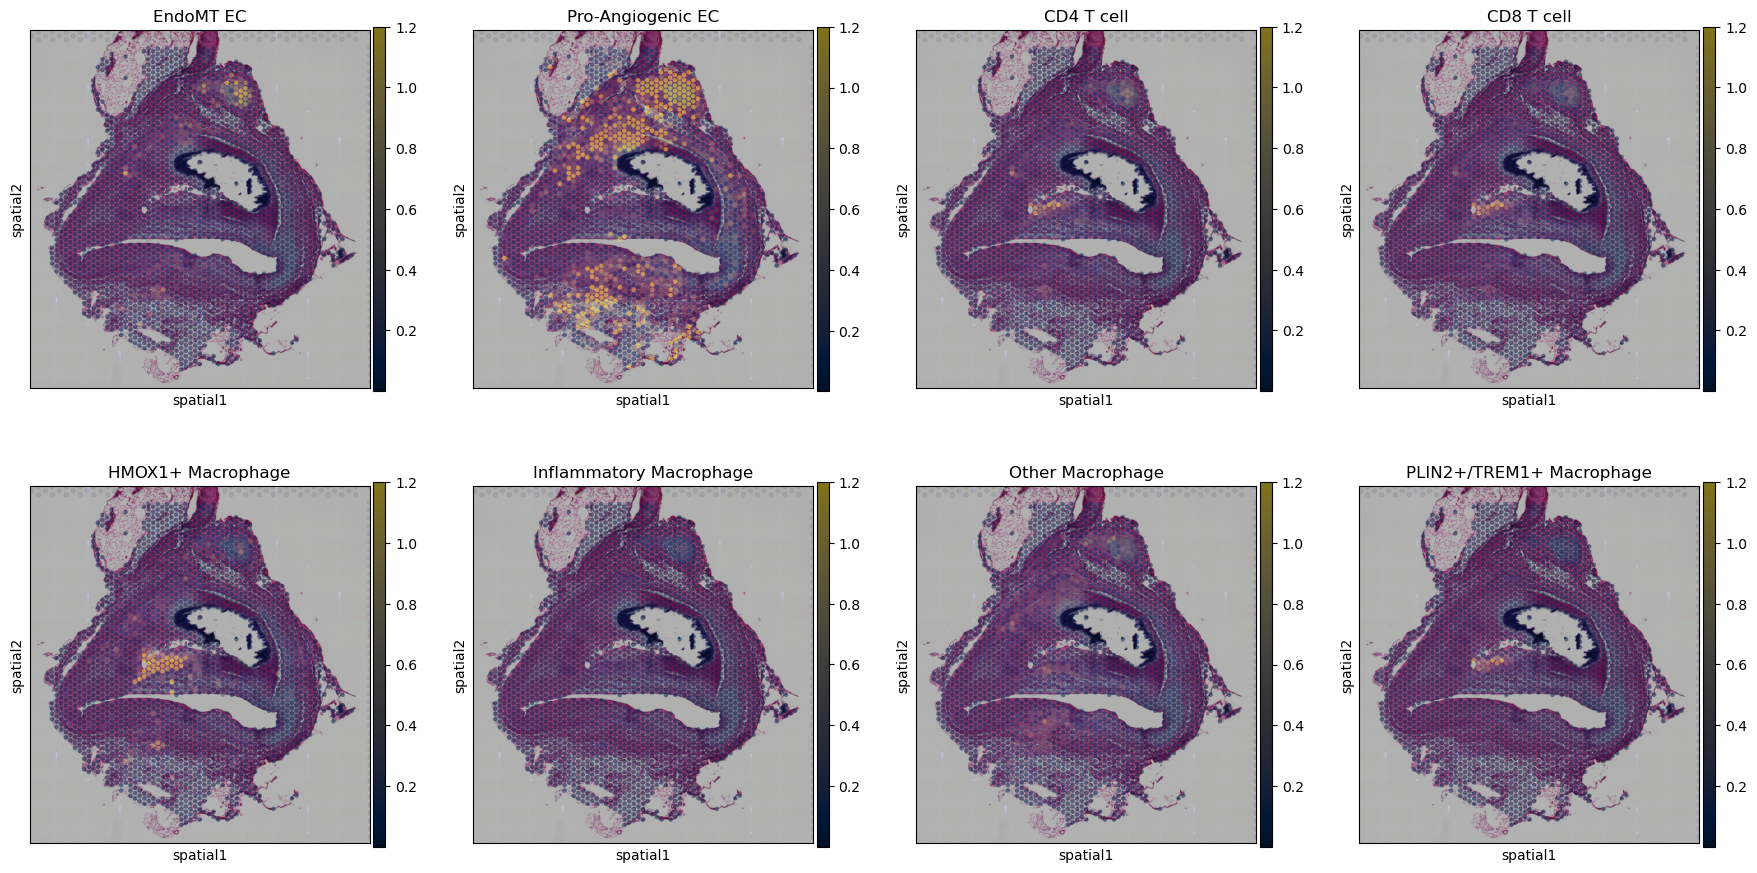
\includegraphics[width=1.1\textwidth]{spatialFibroatheroma2}
    \caption{Spatial cell types for fibroatheroma sample FW104306}
    \label{fig:appendix1}
\end{figure}
\begin{figure}[h]
    \centering
    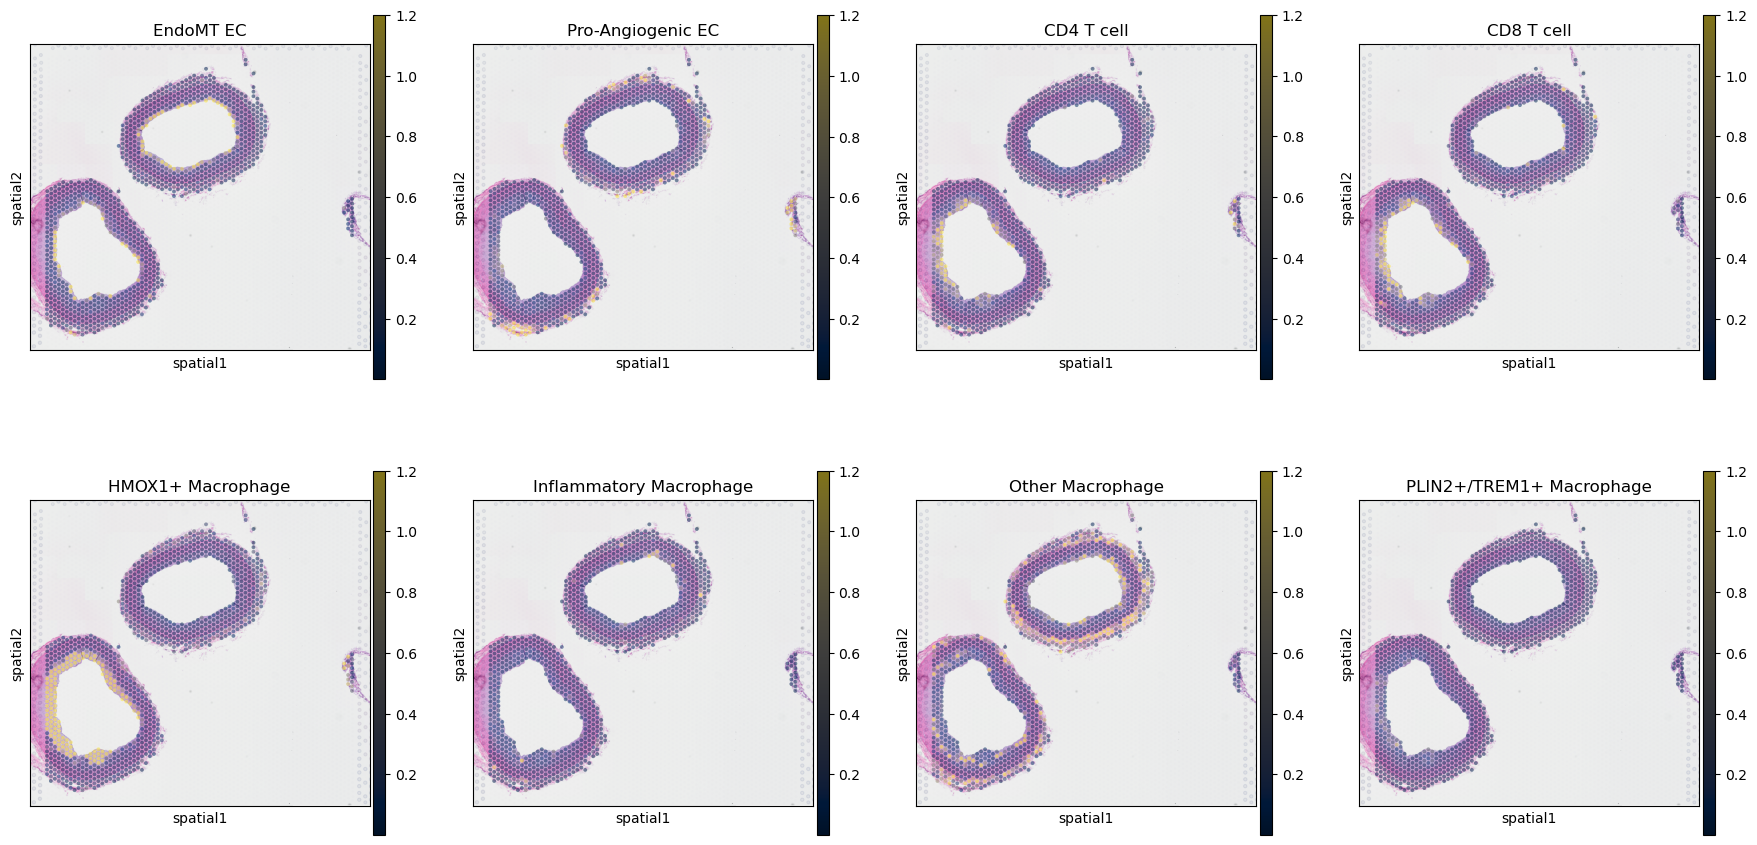
\includegraphics[width=1.1\textwidth]{spatialIntermediateLesion1}
    \caption{Spatial cell types for intermediate lesion sample FW106008}
    \label{fig:appendix1}
\end{figure}
\begin{figure}[h]
    \centering
    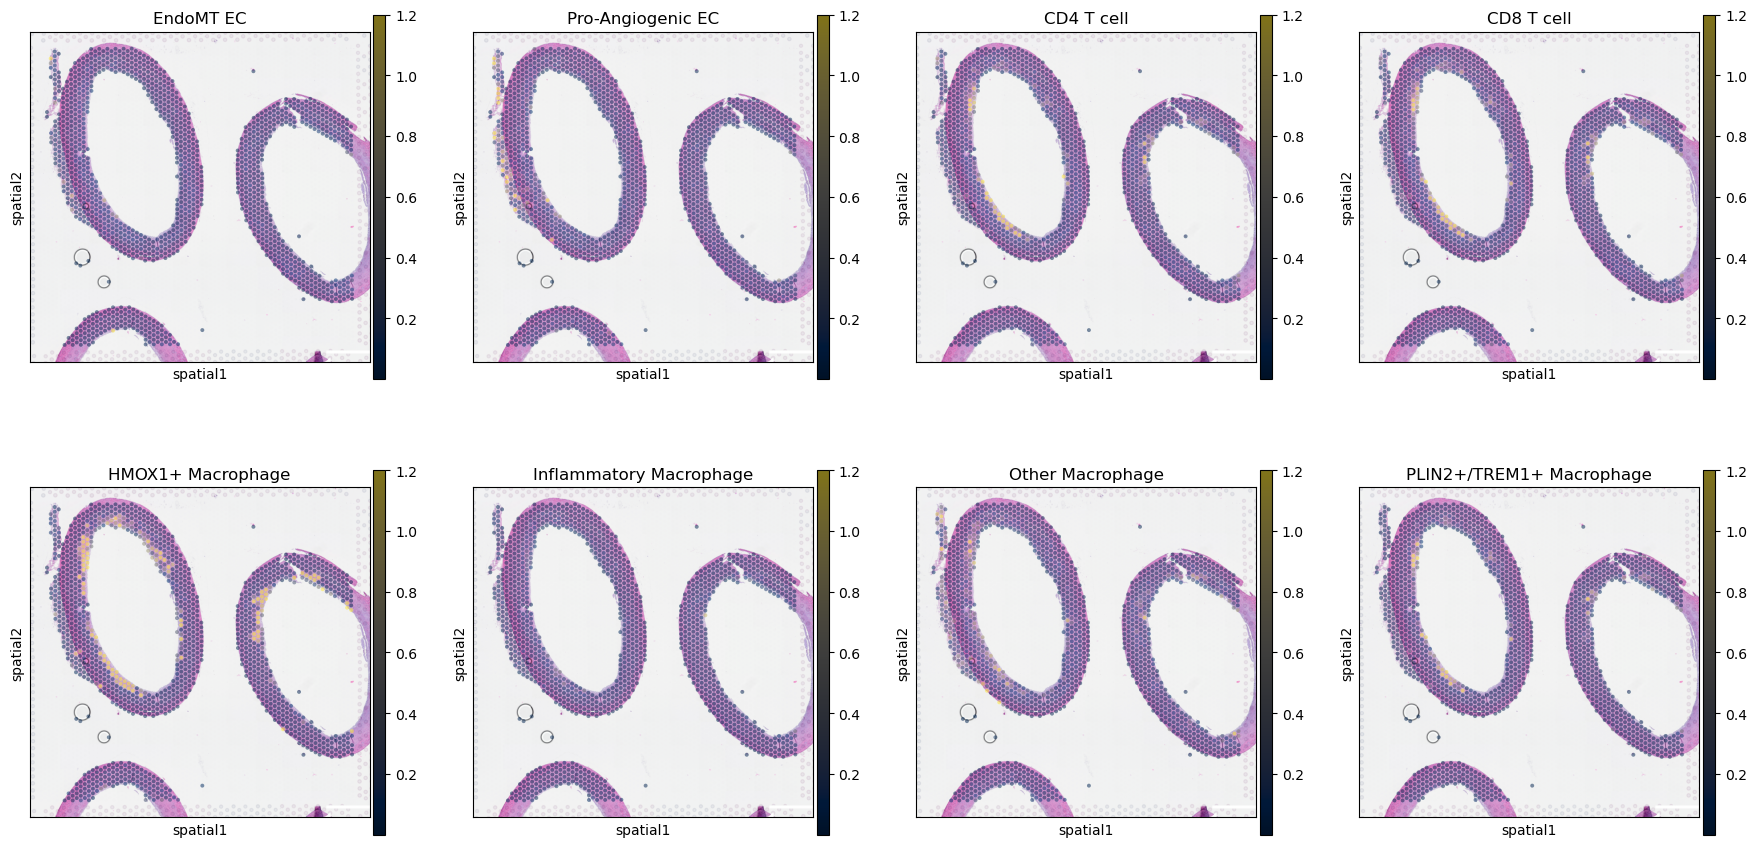
\includegraphics[width=1.1\textwidth]{spatialIntermediateLesion2}
    \caption{Spatial cell types for intermediate lesion sample FW106006}
    \label{fig:appendix1}
\end{figure}
\end{document}
